% ===== 第一部分：单变量分析学 / 第3章：实数的八大基本定理 =====
% !TEX root = ../../main.tex
\setchapterimage{figure/chapter3封面图.png}
\setchapterintro{除了上一章已经讨论过的确界原理与Dedekind定理以外，这一章的讨论重点是剩余的实数基本定理，这一章分为两个部分，基础拓扑与数列，拓扑学部分的一些结论可以迁移到将来的多元函数部分中。这一章的一个问题就是前后的割裂，即使有八大定理的互证作为连接的桥梁，其练习还是有些牵强，我想这也就是为什么一般来说数分中的拓扑学会只涉及直线上与空间中的拓扑。本章的拓扑学部分参考Sydney的Topology without Tears}
\chapter{实数的八大基本定理}
本章我们来考量实数的八大基本定理.

\textbf{定理}：以下8条叙述等价.

\begin{enumerate}
	\item (确界原理)非空有上（下）界数集，必有上（下）确界
	\item （Dedekind 准则）设序对 $(A, A^{\prime})$ 为 $\R$ 的一个分划，则$A$无最大元， $A^{\prime}$ 有最小元．
	\item （单调有界原理）任何单调有界数列必有极限．
	\item （Cantor 区间套定理）若 $\left\{\left[a_n, b_n\right]\right\}$ 是一个区间套，则存在唯一一点 $\xi$ ，使得 $\xi \in\left[a_n, b_n\right], n=1,2, \ldots$ ．
	\item （Bolzano-Weierstrass定理）有界无穷数列必有收敛子列．
	\item （Cauchy 收敛准则）数列 $\left\{a_n\right\}$ 收敛 $\Leftrightarrow$ 对任给的正数 $\varepsilon$ ，总存在某一个自然数 $N$ ，使得 $\forall m, n>N$ 时，都有 $\left|a_m-a_n\right|<\varepsilon$ ．
	
	\item （Heine－Borel 有限覆盖定理）设 $[a, b]$ 是一个闭区间，$H$ 为 $[a, b]$ 上的一个开覆盖，则在 $H$ 中存在有限个开区间，它构成 $[a, b]$ 上的一个覆盖．
	\item （Weierstrass 聚点原理）直线上的有界无限点集至少有一个聚点．
\end{enumerate}

我们先从基础的点集拓扑开始，之后在来讲收敛理论，


\begin{center}
	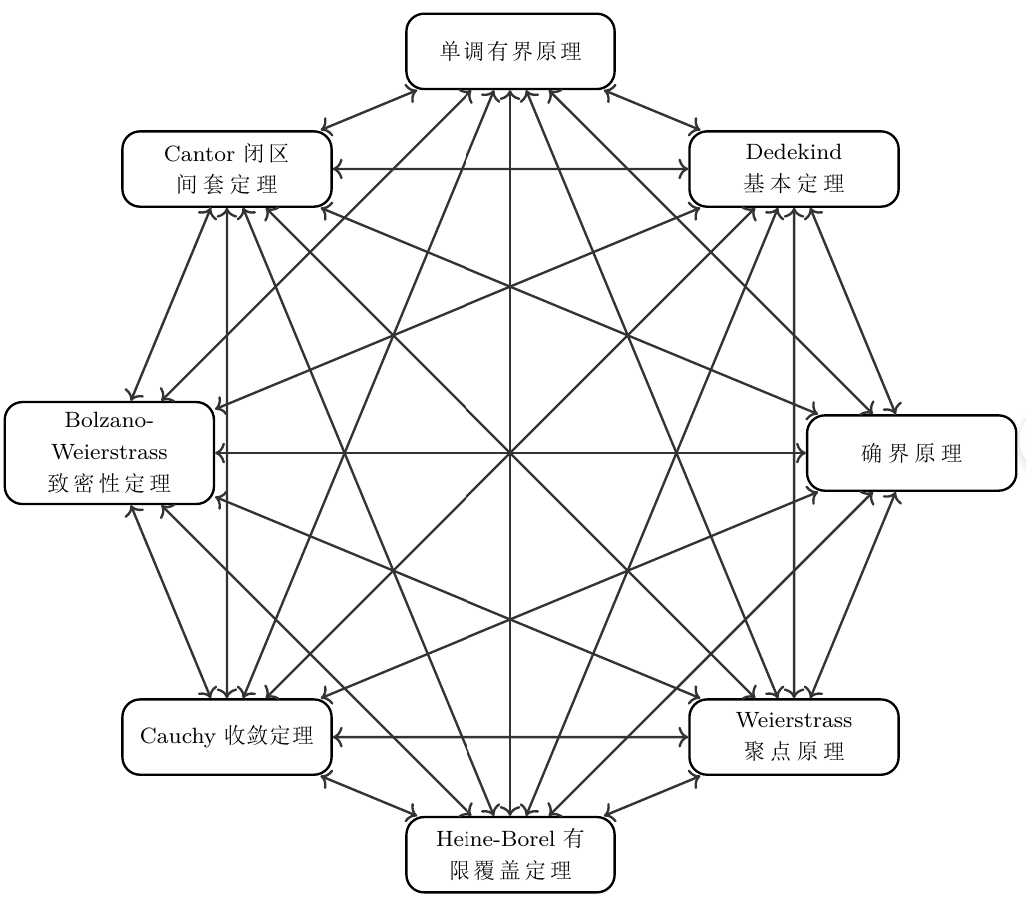
\includegraphics[width=0.6\linewidth]{figure/C2/1}
\end{center}
\newpage
% 第1节：拓扑空间与开闭集
% !TEX root = ../../../main.tex
% 所属：第一部分：单变量分析学 / 第3章：实数的八大基本定理
% 节：3.1 拓扑空间与开闭集
% 正文按原文件顺序保存；由 ../chapter3.tex 调用。
\section{拓扑空间与开闭集}
\begin{definition}\label{defoftosp}
	令$X$是一个集合.$X$的拓扑$\mathcal{T}$是由$X$的一些子集所构成的族，且$\mathcal{T}$满足
	\begin{enumerate}
		\item $X\in \mathcal{T}$且$\varnothing\in\mathcal{T}$
		\item $\mathcal{T}$ 中集合的任意并仍属于 $\mathcal{T}$
		\item $\mathcal{T}$中集合的有限交仍属于$\mathcal{T}$
	\end{enumerate}
	称偶对$\left(\mathrm{X}, \mathcal{T}\right)$ 是一个拓扑空间.
\end{definition}
\begin{definition}
	$\left(\mathrm{X}, \mathcal{T}\right)$ 是一个拓扑空间,那么$\mathcal{T}$中的元素在$\mathrm{X}$中称做开的，换言之$\mathcal{T}$中的元素称为$\mathrm{X}$中的开集.
	
	闭集定义为开集关于$\X$的补集.
	
	在$\left(\mathrm{X}, \mathcal{T}\right)$ 中存在即是开集又是闭集的集，称为闭开集.
\end{definition}
\begin{proposition}
	对拓扑空间$\left(\mathrm{X}, \mathcal{T}\right)$
	
	（1）$\mathrm{X}$ ，$\varnothing$ 是团开的
	
	（2）开集的任意并仍是开集
	
	（3）开集的有限交仍是开集
	
	（4）闭集的任意交仍是闭集
	
	（5）闭集的有限并仍是闭集
\end{proposition}
\begin{proof}
	$(1),(2),(3)$由开集的定义是显然的，对$(4),(5)$使用De Morgan定理,设$S_{\alpha}\in\mathcal{T}$,那么$S_{\alpha}^C$是闭集，则
	$$\bigcap_\alpha S_\alpha^C=\left(\bigcup_\alpha^n S_\alpha\right)^C \text {, 而 }\bigcup_\alpha^n S_\alpha  \in \mathcal{T}$$
	$$	\bigcup_{i=1}^n S_i^C=\left(\bigcap_{i=1}^n S_i\right)^C \text {, 而 } \bigcap_{i=1}^n S_i \in \mathcal{T}$$
\end{proof}
\begin{example}
	\begin{enumerate}
		\item		$\mathrm{X}=  \{a, b, c, d, e, f\}$,令
		$$\mathcal{T}_1=\{\mathrm{X}, \phi,\{a\},\{c, d\},\{a, c, d\},\{b, c, d, e, f\}]$$
		显然地，$\mathcal{T}_1$是$\mathrm{X}$上的一个拓扑：其中
		\begin{itemize}
			\item $\{a\}$是闭开的
			\item$\{b,c\}$既不是闭的，也不是开的是开的，而不是闭的
			\item$\{c,d\}$
			\item$\{a, b, e, f\}$ 是闭的，而不是开的
		\end{itemize}
		\item 离散拓扑$\T$,对集合$\mathrm{X}$,$\T$定义为$\mathrm{X}$所有子集构成的族.显然的，$\mathrm{X}$的任意子集都是闭开的.
		\item 平凡拓扑$\T_0$,定义为
		\[\T_0:=\{\mathrm{X},\varnothing\}\]
	\end{enumerate}
\end{example}
\begin{theorem}
	$f:X\rightarrow Y$,是一个从$X$到$Y$的$1-1$映射，且是满射，令$\left(\mathrm{X}, \mathcal{T}\right)$是一个拓扑空间，设$\T_1=\{f(S):S\in\T\}$,则$\T_1$是$\mathrm{Y}$上的一个拓扑
\end{theorem}
\begin{proof}
	（1）
	
	由 $\mathrm{X} \in \T,  \Y=f(\mathrm{X} )$ 得 $\Y\in \T_1$
	
	由 $\varnothing \in \T,  \varnothing=f(\varnothing)$ 得 $\varnothing \in \T_1$
	
	（2）$A_\alpha \in \T$ ，则 $f\left(A_\alpha\right) \in \T_1$ ，那么考虑
	
	$$
	\bigcup_\alpha f\left(A_\alpha\right)=f\left(\bigcup_\alpha A_\alpha\right) \in \mathcal{T}_1
	$$
	
	(3)$A_n \in \T$则$f\left(A_n\right) \in \T_1$考虑
	
	$$\bigcap_{k=1}^n f\left(A_k\right)=f\left(\bigcap_{k=1}^n A_k\right) \in \T_1$$
\end{proof}
%
% 第2节：Euclidean拓扑与拓扑基
% !TEX root = ../../../main.tex
% 所属：第一部分：单变量分析学 / 第3章：实数的八大基本定理
% 节：3.2 Euclidean拓扑与拓扑基
% 正文按原文件顺序保存；由 ../chapter3.tex 调用。
\section{Euclidean拓扑与拓扑基}
\begin{definition}[$\R$上的Euclidean拓扑]\label{defofeuto}
	$\R$上的一个子集$S$在$\R$上的Euclidean拓扑里被称为是开的，若其有以下性质:
	$$\forall x\in S,\exists a,b\in\R~\textbf{且}~a<b,~\text{使得}~x\in\left(a,b\right)\subset S$$
\end{definition}
注意：在此之后，我们说拓扑空间$\R$,默认为Euclidean拓扑
\begin{proposition}
	\ref{defofeuto}中定义的Euclidean拓扑是一个拓扑
\end{proposition}

\begin{proof}
	（i）$\forall x \in \mathbb{R}$ ，取 $a=x-1, b=x+1,  x \in\left(x-1,  x+1\right)\subset \mathbb{R}$ ，故 $\mathbb{R} \in \T$
	由空真原理，$\varnothing \in \T$
	
	（ii）令 $A_\alpha \in \T$ ，下证 $\bigcup_\alpha A_\alpha \in \T$ ，也即 $\bigcup_\alpha A_\alpha$ 具备\ref{defofeuto}中的性质
	
	取 $x \in \bigcup_\alpha A_\alpha$ ，那么 $\exists k$ ，使得$x \in A_k$ ，$\exists a, b \in \mathbb{R}$ 且 $a<b$ ，使得
	
	$$
	(a, b) \subset A_k \subset \bigcup_\alpha A_\alpha
	$$
	
	
	得证
	
	(iii）考虑 $A_1 \cap A_2$ 的情况，有限交 可以由归纳法得.
	
	取 $A_1, A_2 \in \T$ ，令 $y \in A_1 \cap A_2$ ，则 $y \in A_1, \exists a, b \in \mathbb{R}$ 且 $a<b$ ，使得
	
	$$
	y \in(a, b) \subset A_1
	$$
	
	
	同理 $y \in A_2, \exists c, d \in \mathbb{R}$ ，且 $c<d$ ，s．t．
	$$y \in(c, d) \subset A_2$$
	取 $e=\max \{a, c\}, \quad f=\min \{b, d\}$ ．那么
	
	$$
	y \in(e, f) \subset A_1 \cap A_2
	$$
	
	
	得证
\end{proof}
\begin{proposition}
	对拓扑空间$\R$，我们有以下陈述
	
	（1）开区间$\left(r,s\right)$是开集
	
	（2）区间 $(r,+\infty),(-\infty, r)$ 是开集
	
	（3）闭区间 $[c, d]$ 不是开集而是闭集
	
	（4）单元集 $\{a\}$ 是闭集
	
	（5）$\Z$是闭集
	
	（6）$\Q$不是闭集也不是开集
\end{proposition}
\begin{proof}
	（1）$\forall x \in(r, s)$ ，取 $a=r, b=s$ ，那么 $x \in(a, b) \subset(r, s)$
	
	(2)$\forall x \in(r,+\infty)$ ，取
	
	$$
	x \in(r, x+1) \subset(r,+\infty)
	$$
	
	$\forall y \in(-\infty, r)$ ，取
	
	$$
	y \in(y-1, r) \subset(-\infty, r)
	$$
	
	
	(3)对 $x=c \in[c, d]$ ，假设 $\exists a, b \in \mathbb{R}$ ，使得$c \in(a, b) \subset[c, d]$ ，那么 $a<c<b$ 且 $a<\dfrac{a+c}{2}<c<b$,
	因此 $ \dfrac{a+c}{2} \in(a, b)$ 而 $\dfrac{a+c}{2} \notin[c, d]$ ，矛盾，因此 $[c, d]$ 不是开集.
	
	取 $(-\infty, c) \cup(d,+\infty)$ 为开集，其余集 $[c, d]$ 为闭集
	
	
	(4)考虑$S=\left(-\infty,a\right)\bigcup\left(a,+\infty\right)$为开集，则$S^C=\{a\}$为闭集.
	
	(5)$\Z^C=\bigcup\limits_{n\in\Z}(n,n+1)$是开集，则$\Z$为闭集
	
	(6)若$\Q$为开集，$\left(\forall x\in\Q\right)\left(a,b\in\R\right),$使得$x\in\left(a,b\right)\subset\Q$,$\exists q\in\R\setminus\Q$,同上，$\R\setminus\Q$也不是开集，故$\Q$不是闭集.
\end{proof}
\begin{theorem}
	$\R$的子集$S$是开的，当且仅当$S$是某些开集的并.
\end{theorem}
\begin{proof}
	必要性：$S$ 是开的，$\forall x \in S, \exists I_x=(a, b)$ 使得$x \in I_x \subset S$ 下证
	$$S=\bigcup_{x \in S} I_x$$
	
	（i）$S \subset \bigcup_{x \in S}I_x$
	
	令 $y \in S$ ．则 $y \in I_y \subset \bigcup_{x \in S} I_x$ ，那么 $S \subset \bigcup_{x \in S} I_x$
	
	（ii）$\bigcup_{x \in S }I_x \subset S$
	
	令 $z \in \bigcup_{x \in S} I_x$ ，$\exists t \in S$ ，使得$z \in I_t$ ．而 $I_t \subset S$ ．故 $z \in S$ ，则 $\bigcup_{x \in S} I_x\subset S$
	
	综上
	
	$$
	S=\bigcup_{x \in S} I_x
	$$
	
	
	充分性 :$S=U_{j \in J}\left(a_j, b_j\right)$ ，而$\left(a_j, b_j \right)$开，那么 $S$ 开
\end{proof}
\begin{definition}
	$\left(\X,\T\right)$是一个拓扑空间，由 $\X$ 中的开集组成的族 $\mathcal{B}$被称为是 $\T$ 的基，若 $\X$ 中的任意开集是 $\mathcal{B}$ 中元素的并.
\end{definition}
例：$\R$上的Euclidean拓扑的标准基定义为

$$
\B=\{(a, b): a, b \in \mathbb{R}, a<b\}
$$
也就是$\B$是所有开区间的族.

离散空间$\left(\X,\T\right)$的基可以定义为

$$
\B=\{\{x\}: x \in \X\}
$$

显然易见的，$\T$ 本身是它自己的一个基.若$\B$是 $\T$ 的一个基，$\B_1$ 是一个组，满足 $\B \subset \B_1 \subset \T$ ，那么 $\B_1$ 也是 $\T$ 的一个基.

\begin{proposition}
	\label{eq_of_2def_tpbas}
	令$\X$是一个非空集，且令$\B$是$\X$中某些子集所构成一个族那么 $\B$ 是 $\X$ 的拓扑 $\T$ 的基当且仅当 $\B$ 有如下的性质：
	
	（a）$\X=\bigcup\limits_{B \in \B }B$
	
	（b）$\forall B_1, B_2 \in \B, B_1 \cap B_2$ 是 $\B$ 中元素的并
\end{proposition}


\begin{proof}
	必要性：已知 $\B$ 是$\X$的拓扑 $\T$ 的一个基，那么 $\T$ 满足\ref{defoftosp}中的（i）（ii） （iii）．$\X \in \T$ ，$\X$是开集，根据 $\B$ 的定义$(a)$ ， $(b)$ 得证.
	
	充分性：已知$\B$满足性质（a），（b），使$\T$是由$\B$中元素的并形成的 $\X$ 的所有子集（称$\T$为由$\B$生成的拓扑）
	
	$$
	T=\left\{U \subset \X: U=\bigcup_{B \in \B} B\right\}
	$$
	
	
	下证 $\T$ 是一个拓扑，满足 \ref{defoftosp} 中的（i）（ii）（iii）．
	
	（i）由（a），$\X \in \T$ ，
	而 $\varnothing$ 是 $\B$ 中元素的空并，故$\varnothing \in \mathcal{T}$
	
	（ii）考虑 $T_\alpha \in \T$ ，而每一个 $T_\alpha$ 都为$\B$中元素的并，$\T_\alpha$ 的任意并也为 $\B$ 中元素的并，$\bigcup_\alpha T_\alpha \in \T$
	
	（iii）考虑 $C, D \in \T$ ，则
	
	$$
	C=\bigcup_{k \in K} B_k, D=\bigcup_{j \in J} B_j, K,J \text { 为任意指标集 }
	$$
	
	
	那么
	
	$$
	C \cap D=\left(\bigcup_{k \in K} B_k\right) \cap\left(\bigcup_{j \in J} B_j\right)=\bigcup_{\substack{k \in K \\ j \in J}}\left(B_k \cap B_j\right)
	$$
	
	
	由（b），$C \cap D \in \T$
	
	由归纳法，有限交属于$\T$.
\end{proof}
$\mathbb{R}$ 上闭区间 $[a, b]$ 的 Euclidean 拓扑.
$$\T=\left\{(c, d): a<c<d<b\right\} \cup\left\{[a, e): a<e<b\right\} \cup\left\{(f, b]: a<f<b\right\}$$


$\mathbb{R}^* $ 的 Euclidean 拓扑,其中 $\mathbb{R}^*=[-\infty,+\infty]$
$$\T=\{(a, b):-\infty<a<b<+\infty\}\cup\{[-\infty, c):-\infty<c<-\infty\}\cup\{(d,+\infty]:-\infty<d<+\infty\}$$

$\mathbb{R}^n$ 上的 Euclidean 拓扑的基定义为

$$
\B=\left\{\left(x_1, \cdots, x_n\right) \in \mathbb{R}^n: a_i<x_i<b_i, i=1,2, \cdots, n\right\}
$$
\begin{proposition}
	\label{th:tp_subset}
	对拓扑空间$(\X,\T)$，$\X$的子集构成的族 $\B$ 是 $\T$ 的一个基当且仅当 任对开集 $U$ 中的任何点 $x$ ，存在 $ B \in \B$ 使 得 $x \in B \subset U$ .
\end{proposition}

\begin{proof}
	必要性：已知 $\B$ 是 $\T$ 的一个基，且 $x \in U \in \T$ .由于$U$是一个开集
	
	$$
	U=\bigcup_\alpha B_\alpha, B_\alpha \in \B
	$$
	
	$x \in U$ 则 $\exists j$ ，使得$x \in B_j \subset U$
	
	充分性：已知 $\forall$ 开集 $U$ 中任意点 $x$ ，存在 $B_x \in \B$ 使得 $x \in B_x \subset U$ ，断言
	
	$$
	U=\bigcup_{x \in U} B_x
	$$
	
	
	也即任何开集可以写成 $\B$ 中元素的并.
	
	（i）$U \subset \bigcup_{x \in U} B_x$
	
	$y \in U$ ，$\exists B_y \in B$ 使得$y \in B_y$ ，而 $B_y \subset \bigcup_{x \in U} B_x$ ，故 $y \in U_{x \in U} B_x$ ，即 $U \subset \bigcup_{x\in U} B_x$
	
	（ii）$\bigcup_{x \in U} B_x \subset U$
	
	$z \in \bigcup_{x \in U} B_x$ ，$\exists t \in U$ ，使得$z \in B_t \subset U$ ，故 $z \in U$ ，即 $\bigcup_{x \in U} B_x \subset U$
	
	综上
	
	$$
	U=\bigcup_{x \in U} B_x
	$$
\end{proof}
上面$U=\bigcup_{x \in U} B_x$的证明在以后尝尝用到，我们省略.
\begin{corollary}\label{2.2.8}
	对$(\X,\T)$,$\B$是其拓扑基，那么$\X$的子集$V$是开的当且仅当$(\forall x\in V)(\exists B\in\B),\text{使得}x\in B\subset U$
\end{corollary}
\begin{proof}
	必要性由(\ref{th:tp_subset})得证
	
	充分性:$(\forall x\in V)(\exists B_x\in \B)\text{使得}x\in B\subset V$,那么$V=\bigcup_{x\in V}B_x\in\T$.故$V$是开集
\end{proof}
\begin{corollary}
	$\B_1$ 和 $\B_2$ 分别是 $\T_1$ 和 $\T_2$ 的基，那么 $\T_1=\T_2$ 当且仅当
	
	（i）$\forall B \in \B_1, \forall x \in B, \exists B^{\prime} \in \B_2$ ，使得$x \in B^{\prime} \subset B$
	
	（ii）$\forall B \in \B_2, \forall x \in B, \exists B^{\prime} \in \B_1$ ，使得$x \in B^{\prime} \subset B$
	
\end{corollary}
\begin{proof}
	必要性：$\T_1=\T_2$ ，由 \ref{2.2.8}（i）（ii）易得
	
	充分性：$\B_1, \B_2$ 满足（i）（ii），由\ref{2.2.8}
	（i）说明 $B \in \B_1$ 在 $\left(\X, \T_2\right)$ 上是开的，$\B_1 \subset \T_2$ .因为 $\T_1$ 中的每一个元素都是 $\T_2$ 中元素的并，得 $\T_1 \subset \T_2$ .同理，由（ii）$\T_2 \subset \T_1$
	
	综上 $\T_1=\T_2$
\end{proof}

%
% 第3节：极限点，邻域与连通性
% !TEX root = ../../../main.tex
% 所属：第一部分：单变量分析学 / 第3章：实数的八大基本定理
% 节：3.3 极限点，邻域与连通性
% 正文按原文件顺序保存；由 ../chapter3.tex 调用。
\section{极限点，邻域与连通性}
\begin{definition}\label{defoflimpoint}
	设$A$为拓扑空间$(\X,\T)$的子集，把拓扑空间中的元素称为点，点$x\in\X$称为$A$的极限点(聚点)，若每个包含$x$的开集$U$中包含$A$中不同于$x$的一个点.
\end{definition}
\begin{proposition}
	令 $A$ 为拓扑空间 $(\X, \T)$ 的一个子集. $A$ 在 $(\X, \T)$ 中是闭的当且仅当 $A$ 包含它所有的极限点.
\end{proposition}

\begin{proof}
	必要性：已知 $A$ 在$(\X, \T)$中是闭的.若存在一个 $A$ 的极限点不属于 $A$ ，换言之，存在一个 $A$ 的极限点 $p, p \in A^C$ 且 $A^C$ 是开集，由极限点的定义，$A^C$ 中有一个$A$中不同于 $x$ 的点，矛盾.
	
	充分性：$\forall z \in A^C$ ，$z$ 不是 $A$ 极限点，$\exists$ 开集 $U_z(z\in U_z)$ ，使得．$U_z \cap A=\varnothing$也即 $U_z\subset A^C$ ，因此 $A^C=\bigcup\limits_{z \in A^C} U_z$ ，$A^C$ 是开集的并因此也是开的，因此补集 $A$ 是闭的
\end{proof}
\begin{proposition}
	令$A$为$(\X,\T)$的子集并且$A^{\prime}$是$A$的所有的极限点构成的集合，则$A\cup A^{\prime}$是闭集
\end{proposition}

\begin{proof}
	只需证$A\cup A^{\prime}$包含它本身所有的极限点即可
	
	如不然，$\exists p$是$A\cup A^{\prime}$的极限点，但$p\in(A\cup A^{\prime})^C$
	
	设$p\in(A\cup A^{\prime})^C$，由$p\notin A^{\prime}$,得$p$不是$A$的极限点，$\exists$开集$U,p\in U$,使得
	
	\[U\cap A=\{p\}\text{或}\varnothing\]
	而$p\notin A$,故$U\cap A=\varnothing$
	
	同理，$p$不是$A^{\prime}$的极限点，且$p\notin A^{\prime}$,可以使上述的$U\cap A^{\prime}=\varnothing$
	
	那么$U\cap(A\cup A^{\prime})=\varnothing,p\in U$
	
	如此，$p$不是$A\cup A^{\prime}$的极限点，$A\cup A^{\prime}$是闭集
\end{proof}
\begin{definition}
	$A$ 是 $(\X, \T)$ 的子集，$A^{\prime}$ 是 $A$ 所有极限点的集合，称 $A \cup A^{\prime}$是 $A$ 的闭包，记为 $\bar{A}$
	
	
\end{definition}
\begin{definition}
	$A$ 是 $(\X, \T)$ 的子集，$A$ 在 $\X$ 中处处稠密，若 $\bar{A}=\X$
\end{definition}
\begin{proposition}
	$\mathbb{Q}$ 在 $\mathbb{R}$ 中处处稠密
	
\end{proposition}
\begin{proof}
	只需 $\overline{\mathbb{Q}}=\mathbb{R}$ ，若 $\overline{\mathbb{Q}} \neq \mathbb{R}, \exists x \in \mathbb{R}\setminus \overline{\mathbb{Q}}$ .由 $\mathbb{R}\setminus \overline{\mathbb{Q}}$ 在$\R$中是开的 ,$\exists(a, b) \subset \R\setminus \overline{\mathbb{Q}}$ .但是在每一个$(a, b)$ 存在一个 $ q \in \mathbb{Q}$ ，那么
	
	$$
	q \in(a, b) \subset \mathbb{R}\setminus \overline{\mathbb{Q}} \Rightarrow q \subset \mathbb{R}\setminus \mathbb{Q}
	$$
	
	
	矛盾.
\end{proof}
显然地，若 $A$ 在 $\X$ 中稠密则 $A^C$ 中全部是 $A$ 的极限点.
\begin{proposition}
	$A$ 是$(\X,\T)$的子集，$A$ 在 $\X$ 中稠密当且仅当 $\forall U \in \T$且 $U\neq \varnothing, A \cap U \neq \varnothing$
\end{proposition}

\begin{proof}
	必要性：已知 $A$ 在$\X$中处处稠密，则 $A \cup A^{\prime}=\X$
	
	假设 $U \cap A=\varnothing . \forall x \in U, x \notin A$ 则 $x$ 不是 $A$ 的极限点，这与 $A^C$ 中全部是 $A$的极限点矛盾.
	
	充分性：己知 $\forall U \in\T$ 且 $U \neq \varnothing, A \cap U \neq \varnothing$
	
	若 $A=\X$ ，显然 $A$ 在$\X$中稠密
	
	若 $A \neq \X$ ，设 $x \in A^C$ .如果 $U \in \T$ ，且 $x \in U$ ，那么 $U \cap A \neq \varnothing$ ，于是 $x$ 是 $A$ 的一极限点. $\forall x \in A^C$ ，$x$ 都是 $A$ 的极限点，也即 $x \in A^{\prime}$ ，于是 $A^C \subset A^{\prime}$ ，则 $\bar{A}=A^{\prime} \cup A=\X$
	
\end{proof}
\begin{definition}
	$(\X,\T)$是一个拓扑空间，$N$ 是 $
	\X$ 的子集且 $p \in N$ .若对 $p$ ，存在一个开集$U$，使得，$p \in U \subset N$ ，称 $N$ 为 $p$ 的邻域.
\end{definition}
\begin{proposition}
	$A$ 是$(\X,\T)$的子集，点 $x \in \X$ 是 $A$ 的极限点当且仅当 $x$ 的每个邻域包含一个不同于$\X$属于$A$的点
	
\end{proposition}

\begin{proof}
	根据定义显然
\end{proof}
\begin{corollary}
	
	（1）$A$ 是 $(\X, \T)$ 的子集，$A$ 是闭的当且仅当 $\forall x \in A^C$ ，$\exists x$ 的邻域 $N$满足 $N \subset A^C$
	
	（2）$U$是$(\X, \T)$ 的子集，$U$是开的当且仅当 $\forall x \in U$ ，$\exists x$ 的邻域满足$N\subset U$
	
	（3）$U$是$(\X, \T)$ 的子集，$U \in \T$ 当且仅当 $\forall x \in U, \exists V \in \T$ ，使得$x \in V\subset U$
\end{corollary}
\begin{definition}
	在 $\mathbb{R}$ 上，球型邻域定义为
	
	$$
	\left(x_0-\delta, x_0+\delta\right)
	$$
	
	
	记为 $N\left(x_0, \delta\right)$ 或 $O\left(x_0, \delta\right)$ 
	
	下文中，在 $\mathbb{R}$上 的邻域默认为球型邻域
\end{definition}
\begin{lemma}
	$S$是$\R$上有界的子集，$S$是闭的则$p=\sup S\in S$
\end{lemma}
\begin{proof}
	设$p\in S^C$,$S^C$是开的，故$\exists(a,b)$,使得$p\in(a,b)\subset S^C$
	
	$p=\sup S$,而$a<p$.$\exists x\in S$,使得$x>a$,且$x<p<b$,那么$x\in(a,b)\subset S^C$,矛盾
\end{proof}
\begin{definition}
	对$(\X,\T)$,称$X$是连通的，若闭开集只用$\X$与$\varnothing$
\end{definition}
\begin{proposition}
	\label{con_of_R}
	$\R$是连通的
\end{proposition}

\begin{proof}
	也即 $\mathbb{R}$ 上的闭开集只有 $\mathbb{R}$ 与 $\varnothing$
	
	假设 $T \neq \mathbb{R}$ 且 $T \neq \varnothing$ ，且$T$ 是闭开的. $\exists x \in T,  z \in T^c$
	不失一般性， 假设 $x<z$ .令 $S=T \cap[x, z]$ ，$S$ 是闭的.
	
	$z$ 是 $S$ 的上界，$S$ 有上确界，令 $p=\sup S$ ，故 $p \in S$ ，因此 $p \in[x, z], p \leqslant z$，又 $p \in T, z \in T^c, p \neq Z$ 故 $p<Z$ .
	
	又 $T$ 是开集，$p \in T . \exists(a, b), p \in(a, b)\subset T$
	
	取 $t$,使得$p<t<\min (b, z)$ ，有 $t \in T$ 且 $t \in[p, z]$
	
	因此 $t \in T \cap[x, z]=S$ ，而 $t > p=\sup S$ ，矛盾
	
	故 $T=\mathbb{R}$ 或 $\varnothing$
\end{proof}

%
% 第4节：同胚关系与同胚映射
% !TEX root = ../../../main.tex
% 所属：第一部分：单变量分析学 / 第3章：实数的八大基本定理
% 节：3.4 同胚关系与同胚映射
% 正文按原文件顺序保存；由 ../chapter3.tex 调用。
\section{同胚关系与同胚映射}

\begin{definition}
	令 $Y$ 是 拓扑空间 $(\X, \T)$ 的一个非子集.族 $\T_Y=\{O \cap Y: O \in \T\}$ 由 $Y$ 的子集组成，是一个定义在 $Y$ 上的拓扑,称之为子空间拓扑，$\left(Y, \T_Y\right)$ 称为 $(\X, \T)$ 的子空间
\end{definition}
\begin{definition}
	对$(\X,\T_1),(Y,\T_2)$,若函数$f:\X\rightarrow Y$满足：
	
	（i）$f$ 是$1-1$的且是满射
	
	（ii）$\forall U \in \T_2, f^{-1}(U) \in \T_1$
	
	（iii）$\forall V \in \T_1, f(V) \in \T_2$
	
	就称 $\left(x, \T_1\right),\left(Y, \T_2\right)$ 是同胚的.称 $f$ 是 $\left(\X, \T_1\right),\left(Y, \T_2\right)$ 之间的一个同胚映射，记为 $\left(\X, \T_1\right)\cong\left(Y, \T_2\right)$
\end{definition}
\begin{proposition}
	同胚关系是一个等价关系.
\end{proposition}
\begin{proof}
	应有
	
	（1）$\left(\X, \T_1\right) \cong\left(\X, \T_1\right)$
	
	(2)$\left(\X, \T_1\right) \cong\left(Y, \T_2\right) \Leftrightarrow\left(\Y, \T_2\right) \cong\left(\X, \T_1\right)$
	
	（3）$\left(\X, \T_1\right) \cong\left(Y, \T_2\right),\left(Y, 
	\T_2\right) \cong\left(Z, \T_3\right) \Rightarrow\left(\X, \T_1\right) \cong\left(Z, \T_3\right)$
	
	只需验证恒等映射，逆映射，复合映射满足（i），（ii），（iii）即可.显然地，得证
\end{proof}
\begin{example}
	
	(a) $(0,1) \cong(a, b)$
	
	(b) $(-1,1) \cong \mathbb{R}$
	
	(c) $[a, b] \cong \mathbb{R}^*$
	
	(d) $[c, d) \cong(c, d]$
\end{example}
\begin{proof}
	（a）$f(x)=a(1-x)+b x$
	
	（i）显然地，$f$ 是 $1-1$ 的，且为满射
	
	
	(iii)	$$\begin{aligned}
		f((0,1) \text { 中开集}) & =f((0,1) \text { 中开区同的并 }) \\
		& =(a, b) \text { 中开区间的并 } \\
		& =(a, b) \text { 中开集 }
	\end{aligned}
	$$
	
	
	对（ii）考查 $f^{-1}$ 即可.
	
	故 $f$ 是 $(0,1) \rightarrow(a, b)$ 上的同胚映射.
	
	故 $(0,1) \cong(a, b)$
	
	（b）$$f(x)=\dfrac{x}{1-|x|}$$
	
	（c）考虑 $\left[-\dfrac{\pi}{2}, \dfrac{\pi}{2}\right]$ ，易知 $[a, b] \cong\left[-\dfrac{\pi}{2}, \dfrac{\pi}{2}\right]$
	
	$$
	\begin{gathered}
		f(x)=\tan ^{-1}(x) \quad x \in \mathbb{R}^* \\
		f: \mathbb{R}^* \rightarrow\left[-\dfrac{\pi}{2}, \dfrac{\pi}{2}\right]
	\end{gathered}
	$$
	
	（d）$f(x)=c+d-x$\end{proof}
\begin{theorem}
	同胚于连通空间的拓扑空间是连通的
\end{theorem}
\begin{proof}
	设 $\left(\X, \T_1\right) \cong\left(\Y, \T_2\right)$ ，已知 $\left(\X, \T_1\right)$ 连通，
	
	设 $\left(\Y, \T_2\right)$ 不连通，$\exists Y_1 \subset Y, Y_1 \neq Y$ 或 $\varnothing$ ，使得$Y_1$ 是闭开的，则 $f^{-1}\left(Y_1\right) \subset \X$ ，是 $\X$ 的闭开子集，矛盾，故 $\left(Y, \T_2\right)$ 连通 
\end{proof}

\begin{definition}
	$\mathbb{R}$ 中的子集 $S$ 称为区间，若它满足如下性质：也果 $x \in S$ ， $z \in S, y \in \mathbb{R}$ ，使得$x<y<z$ ，那 么$ y \in S$
\end{definition}

每个区间具下列形式之一：
\[\{a\},[a, b],(a, b),[a, b),(a, b],(-\infty, a),(-\infty, a],(a,+\infty),[a,+\infty),(-\infty,+\infty)\]

\begin{proposition}\label{2.4.7}
	$\R$的子空间$S$是连通的当且仅当$S$是一个区间
\end{proposition}
\begin{proof}
	充分性：证明类似于\ref{con_of_R} 略
	
	必要性：S是连通的，假定 $x \in S,  z \in S,  x<y<z$ ，且 $y \notin S$ .
	
	则 $(-\infty, y) \cap S=(-\infty, y] \cap S$ ，是 $S$ 的闭开子集,需证 $(-\infty, y) \cap S$ 是真且非空子集.由 $x \in S, x<y$ 得 $x \in(-\infty, y) \cap S$ ，它是真子集.由于 $z \in S$ ，但 $z \notin(-\infty, y) \cap S$ 于是 $S$ 不连通，矛盾
\end{proof}
\begin{theorem}
	$f:\left(\X, \T_1\right) \rightarrow\left(Y, T_2\right)$ 是同胚映射，令$a \in X$ ，考虑 $x\setminus \{a\}$与其子空间拓扑 $\T_1^{\prime}$ ，对 $f(a)$ ，考虑$Y\setminus \{f(a)\}$ 与其子空间拓扑 $\T_2^{\prime}$ ，则$(\X\setminus \{a\}, \T_1^{\prime})\text{与}\left(Y\setminus \{f(a)\}, \T_2^{\prime}\right)$ 同胚
\end{theorem}
\begin{proof}
	构造 $g:\left(X\setminus \{a\}, \T_1^{\prime}\right) \rightarrow\left(Y\setminus \{f(a)\}, \T_2^{\prime}\right)$ 即可，$g=f(x \neq a)$容易得$g$是一个同胚映射.
	
	
\end{proof}
\begin{corollary}
	
	（i）$(a, b)$不同胚于$[c, d)$
	
	（ii）$(a, b) $不同胚于 $[c, d]$
	
	（iii）$[a, b)$不同胚于$[c, d]$
	
\end{corollary}
\begin{proof}
	（i）：$X=[c, d),  Y=(a, b)$ ，假设 $X \cong Y$
	考虑 $X\setminus \{c\} \cong Y\setminus \{y\}$
	那么 $(c, d)$ 是一个区间，由\ref{2.4.7}, $(c, d)$ 是连通的，且 $Y\setminus \{y\}$ 是连通的，但 $(a, b)$ 去掉任何一个点都会导致它不连通，故$\X$不同胚于$Y$
	（ii），（iii）同理
\end{proof}
%
% 第5节：度量空间
% !TEX root = ../../../main.tex
% 所属：第一部分：单变量分析学 / 第3章：实数的八大基本定理
% 节：3.5 度量空间
% 正文按原文件顺序保存；由 ../chapter3.tex 调用。
\section{度量空间}
\begin{definition}
	$\X$ 是一个非空集，$d$ 是一个映射，定义在 $\X \times \X$ 上，$\forall a, b \in \X$ ，若满足
	
	（i）若 $a \neq b$ ，那么 $d(a, b)>0 ; d(a, a)=0$
	
	（ii）$d(a, b)=d(b, a)$
	
	（iii）$d(a, c) \leqslant d(a, b)+d(b, c)$
	
	那么 $d$ 称为 $\X$ 上的一个度量或者距离函数，$(\X, d)$ 称为度量空间. $d(a, b)$ 称为$a, b$ 之间的距离
\end{definition}
在$\R$上\[d(a,b)=|a-b|\]
称为$\R$上的Euclidean度量

在$\R^2$\[d((a_1,a_2),(b_1,b_2))=\sqrt{(a_1-b_1)^2+(a_2+b_2)^2}\]称为$\R^2$上的Euclidean度量
\begin{definition}
	令$(\X,d)$是一个度量空间，$r$ 是任意正实数.集合
	
	$$
	B_r(a)=\{x: x \in \X \text { 且 } d(a, x)<r\}	$$
	
	
	称为以 $a$ 为中心，$r$ 內为半径的开球
\end{definition}
\begin{lemma}
	令 $(\X, d)$ 是一个度量空间，且 $a, b \in \X . \delta_1, \delta_2 \in \mathbb{R}_{+}$若 $c \in B_{\delta_1}(a) \cap B_{\delta_2}(b), \exists \delta>0$ ，使得，$B_\delta(c) \subset B_{\delta_1}(a) \cap B_{\delta_2}(b)$
\end{lemma}
\begin{proof}
	取 $\delta=\min \left\{\delta_1-d(c, a), \delta_2-d(c, b)\right\}$ 即可
\end{proof}
\begin{corollary}\label{ints_of_ball}
	$(\X, d)$ 是一个度量空间，$B_1, B_2$ 是$(\X,d)$中的开球那么 $B_1 \cap B_2$ 是 $(X, d)$ 中一些开球的并集
\end{corollary}
\begin{proof}
	$\forall c \in B_1 \cap B_2$（假设不为 $\varnothing, \varnothing$ 下平凡）.
	
	$\exists \delta(c)$ ，使得，$B_{\delta(c)}(c) \subset B_1 \cap B_2$ ，
	
	那么
	
	$$
	B_1 \cap B_2=\bigcup_{x \in B_1 \cap B_2} B_{\delta(x)}(x)
	$$
\end{proof}
显然的，我们有以下的命题
\begin{proposition}
	令 $(\X, d)$ 是一个度量空间．那么 $(\X, d)$ 中所有开球构成一个族，是$\X$中一个拓扑的拓扑基
\end{proposition}
\begin{proof}
	由\ref{eq_of_2def_tpbas}与\ref{ints_of_ball}得
\end{proof}
称$\T$为度量$d$诱导出的拓扑
\begin{proposition}
	$(\X,d)$是一个度量空间，$\T$是由$d$诱导出的拓扑，$(\X,\T)$的子集$U$是开的，当且仅当$(\forall a\in U)(\exists \varepsilon>0),$使得$B_\varepsilon(a)\subset U$
\end{proposition}
\begin{proof}
	必要性：$U \in\T$ ，所有开球是一个拓扑基.
	
	$$
	U=\bigcup_{x \in U} B_{\delta(x)}(x)
	$$
	
	
	对 $a, \varepsilon=\delta(a), a \in B_{\varepsilon}(a) \subset U$
	
	充分性：这等价于 $\quad U=\bigcup_{a \in U} B_{\varepsilon(a)}(a)$
	
	说明$U$是开的.
\end{proof}
\begin{definition}
	$(\X,\T)$是一个拓扑空间，$A$是其任意子集. $A$ 包含的最大的那个开集称为 $A$ 的内部，记为 $\operatorname{Int}(A)$ . $\forall x \in \operatorname{Int}(A), x$ 称为 $A$ 的内点.
	
	$\operatorname{Int}\left(A^c\right)$ 定义为 $A$ 的外部，其任何点称为 $A$ 的外点，外部记为$\operatorname{Ext}A $
	
	$A$ 的边界定义为 $\bar{A}\setminus\operatorname{In} t(A)$ ，记为 $\partial A$ ，其点称为 $A$ 的边界点
\end{definition}

%
% 第6节：紧集，Cantor集与Heine-Borel定理
% !TEX root = ../../../main.tex
% 所属：第一部分：单变量分析学 / 第3章：实数的八大基本定理
% 节：3.6 紧集，Cantor集与Heine-Borel定理
% 正文按原文件顺序保存；由 ../chapter3.tex 调用。
\section{紧集，Cantor集与Heine-Borel定理}
\begin{definition}
	$\mathcal{O}=\left\{O_i\right\}$是$\X$子集构成的族，$i \in I$ ，$I$是指标集．$A$是 $\X$的一个子集.则若
	
	$$
	A \subset \bigcup_{i \in I} O_i
	$$
	
	
	称 $O_i, i \in I$ 为 $A$ 的覆盖.
	
	若上述定义中的 $O_i$ 为 $(\X, \T)$ 中的开集，则 $O_i, i \in I$ 称为 $A$ 的一个开覆盖.
	
	将$O_i, i \in I$ 的有限子族$O_{i_1}, O_{i_2}, \cdots, O_{i_n}$  称 $A$ 的有限子覆盖.若 $A \subset O_{i_1} \cup O_{i_2} \cup \cdots \cup O_{i_n}$
\end{definition}
\begin{definition}
	$(\X,\T)$的子集$A$被称为是紧的，若$A$的任意开覆盖存在一个有限子覆盖.
	
	若$(\X,\T)$的紧子集$A=\X$,则称$(\X,\T)$是紧空间
\end{definition}
\begin{proposition}
	$f:(\X,\T_1)\rightarrow(\Y,\T_2)$是一个同胚映射，若$(\X,\T_1)$是紧空间，则$(\Y,\T_2)$紧空间.
\end{proposition}
\begin{proof}
	$\forall\left\{U_i\right\}_{i\in I}$ 使得，
	$$U_i \in \T_2$$且 $$\Y \subset \bigcup_{i \in I} U_i$$
	
	由 $f$是一个同胚，$f^{-1}\left(U_i\right) \in \T_1$,$\forall x \in \X, f(x) \in \Y . f(x)$ 必属于某 $U_j$ ，故 $x \in f^{-1}\left(U_j\right)$
	于是 $\left\{f^{-1}\left(U_i\right)\right\}_{i \in I}$ 是$\X$的一个开覆盖.
	
	由$X$紧，存在有限子覆盖.
	$$\X\subset f^{-1}(U_{i_{1}})\cup\cdots\cup f^{-1}(U_{i_{n}})$$
	则
	$$\Y=f(\X)\subset U_{i_{1}}\cup\cdots\cup U_{i_{n}}$$
	
	
	于是$\Y$是紧空间.
	
\end{proof}
\begin{theorem}[Heine-Borel 定理]\label{HB_Th}
	$\R$的子集是紧的当且仅当该子集为有界闭集
\end{theorem}
在证明\ref{HB_Th}之前我们先做一些准备工作.
\begin{proposition}
	$\left[0,1\right]$是紧的
\end{proposition}
\begin{proof}
	$O_i, i \in I$ 是 $[0,1]$ 的一个开覆盖. $\forall x \in[0,1], \exists O_i$ 使得$x \in O_i$ ．而$O_i$是开的,存在在 $[0,1]$ 中开的区间 $U_x$，使得$x \in U_x \subset O_i$
	
	定义 $[0,1]$ 的子集 $S$：
	$$S=\left\{z:\left[0, z\right] \textbf{可以被有限个} U_x \textbf{覆盖} \right\}$$
	也即 $z \in S \Rightarrow\left[0, z\right] \subset U_{x_1} \cup U_{x_2} \cup \cdots \cup U_{x_n}$ ,对某些 $x_1, \cdots, x_n$ 
	
	现在，令 $x \in S$ 和 $y \in U_x$ .那么 $U_x$ 是一个包含 $x$ 和 $y$ 的区间.
	
	$[x, y] \subset U_x .(\textbf{不失一般性} x \leqslant y)$ 所以
	
	$$
	[0, y] \subset U_{x_1} \cup U_{x_2} \cup \cdots \cup U_{x_n} \cup U_x
	$$
	
	
	因此 $y \in S$ ．
	
	$
	\forall x \in[0,1], U_x \cap S=U_x \text { 或 } \varnothing
	$
	
	
	这说明
	
	$$
	S=\bigcup_{x \in S} U_x
	$$
	
	
	并且
	
	$$
	[0,1]\setminus S=\bigcup_{x \notin S} U_x
	$$
	
	
	因此，$S$ 既是开的，也是闭的在 $[0,1]$ 中，由 $[0,1]$ 的连通性，$S=[0,1]$ 或 $\varnothing$
	
	而 $0 \in S$ ，故 $S=[0,1]$ ，这就是说 $[0,1]$ 可以被有限个 $U_x$覆盖.故 $[0,1] \subset U_{x_1} \cup \cdots \cup U_{x_m} \subset O_{i_1} \cup \cdots \cup O_{i_m}$ ，因此 $[0,1]$ 是紧的.
	
	
\end{proof}
由同胚映射对紧性的保持，$\left[a,b\right]$也是紧的.
\begin{proposition}
	任何紧空间的闭子集都是紧的.
\end{proposition}
\begin{proof}
	令 $A$ 是紧空间$(\X,\T)$的一个闭子集.今 $U_i \in \T, i \in I$ 是 $A$ 的任意开覆盖,那么
	
	$$
	\X \subset\left(\bigcup_{i \in I} U_i\right) \cup(\X\setminus A)
	$$
	
	
	而$\X$紧，故存在 $i_1, \cdots, i_k $使得
	
	$$
	\X \subset U_{i_1} \cup U_{i_2} \cup \cdots \cup U_{i_k} \cup(X\setminus A)
	$$
	
	
	那么
	
	$$
	A \subset U_{i_1} \cup U_{i_2} \cup \cdots \cup U_{i_k}
	$$
	
	
	因$A \cap(X\setminus A)=\varnothing$ ,故 $A$ 是紧的
\end{proof}
现在我们回归到\ref{HB_Th}的证明
\begin{proof}
	对有界闭的集合 $A$ ，必存在区间 $[a, b]$ ，使得$A \subset[a, b]$, $A$是紧空间$\left[a,b\right]$的闭子集,故$A$是紧的.
	
	下面,已知$A$是$\R$的紧子集，证明$A$是有界闭集
	
	$(i)$紧$\Rightarrow$有界
	
	A是紧的，取开覆盖
	
	$$
	\{(-n, n): n \in \mathbb{N}\}
	$$
	
	
	存在有限子覆盖
	$$A \subset\left(-n_1, n_1\right) \cup \cdots \cup\left(-n_k, n_k\right)$$
	令 $N=\max \left\{n_1, \cdot, n_k\right\}$．
	
	$$A \subset(-N, N) \subset \left[-N,N\right]$$
	故A有界.
	
	$(ii)$紧$\Rightarrow$闭
	
	只需证 $A$ 包含其所有极限点，也即若 $x \notin A$ ，则存在包含 $x$ 的开集与 $A$交集为空集.
	
	取定 $x \notin A$ ，对每个 $y \in A$ ，令 $\varepsilon_y=\dfrac{|x-y|}{2}>0$
	取开集
	
	$$
	U_y=\left(y-\varepsilon_y, y+\varepsilon_y\right), \quad V_y=\left(x-\varepsilon_y, x+\varepsilon_y\right)
	$$
	
	
	则 $U_y \cap V_y=\varnothing$
	
	$\left\{U_y\right\}_{y \in A}$ 是 $A$ 的一个开覆盖.由 $A$ 的紧性，存在有限子覆盖，
	
	
	$$
	A \subset U_{y_1} \cup U_{y_2} \cup \cdots \cup U_{y_n}
	$$
	再令
	
	$$
	V=V_{y_1}\cup V_{y_2}\cup \cdots \cup V_{y_n}
	$$
	
	
	$V$是开集且$x \in V$ .
	
	
	$\forall z \in A, \exists j$ ,使得 $z \in U_{y_j}$而, $U_{y_j} \cap V_{y_j}=\varnothing$ ,故 $z \notin V_{y _j}$ 从而 $z \notin V$因此 $A \cap V=\varnothing$
	
	于是我们找到了$x$一个邻域且与$A$不交,故$A$为闭集.
\end{proof}

Heine-Borel定理在$\R^n$上依旧成立,这一点我们在多元分析的部分中讨论.

回顾我们已经做的，
\[\text{确界原理}\Rightarrow\text{连通性定理}\Rightarrow\text{Heine-Borel定理}\]
下面，我们证明这三者等价，只需证明$\text{Heine-Borel定理}\Rightarrow\text{确界原理}$
\begin{theorem}
	$\text{Heine-Borel定理}\Rightarrow\text{确界原理}$
\end{theorem}
\begin{proof}
	$S$是一个上有界的集合,设其一个上界为$b$,任取$a\in S$,考察区间$\left[a,b\right]$.假设$S$无上确界，对$\left[a,b\right]$中的元素$x$,分别构造开集
	
	\begin{enumerate}
		\item$U\subset\left[a,b\right]\cap S$,若$x\in U$
		
		因$S$无上确界，$\exists y_x>x\textbf{且}y_x\in S$,自然的$y_x\in U$,令$\delta_x=\dfrac{y_x-x}{2}$,取$\left(x-\delta_x,x+\delta_x\right)$,令
		$$U_x=\left(x-\delta_x,x+\delta_x\right)\cap\left[a,b\right] ,U_x\subset U,\textbf{不含S的上界}$$
		
		\item$U^C=\left[a,b\right]\setminus U$,若$x\in U^C$
		
		因$S$无上确界,$U^C$无最小下界，$\exists z_x<x\textbf{且}z_x\in U^C$,令$\delta_x=\dfrac{x-z_x}{2}$,取$\left(x-\delta_x,x+\delta_x\right)$,令
		$$U_x=\left(x-\delta_x,x+\delta_x\right)\cap\left[a,b\right] ,U_x\subset U^C,\text{只含S的上界}$$
	\end{enumerate}
	这样，我们得到了一个$\left[a,b\right]$的开覆盖$\left\{U_x\right\},x\in\left[a,b\right]$,其中$U_x$要么全是上界，要么完全不含上界.
	
	有Heine-Borel定理，有有限子覆盖，$\left\{U_{x_i}\right\}_{i=1}^n$,$\left[a,b\right]\subset \bigcup_{i=1}^n U_{x_i}$
	
	从$b$开始，$\exists U_{x_k}=(c_1,b]$,使得$b\in U_{x_k}$,不失一般性的，设$k=1$
	
	$b\in U_{x_1}$,且$U_{x_1}$中只包含$S$的上界，根据$U_{x_1}$的构造方式，$c_1\in U^C$
	
	对$c$,$\exists U_{x_2}=\left(c_2,d_2\right)$,使得$c_1\in U_{x_2}$,$U_{x_2}$中只包含$S$的上界,$c_2\in U^C$.
	
	不断向左进行，在有限次内，必可以使$a\in U_{x_j}$且$U_{x_j}$只包含$S$的上界，与$a\in S$矛盾
\end{proof}














%
% 第7节：数列的极限与其性质
% !TEX root = ../../../main.tex
% 所属：第一部分：单变量分析学 / 第3章：实数的八大基本定理
% 节：3.7 数列的极限与其性质
% 正文按原文件顺序保存；由 ../chapter3.tex 调用。
\section{数列的极限与其性质}
\begin{definition}
	称$\left\{x_n\right\}$ 收敛于 $a$ ，若满足
	$$
	\begin{gathered}
		\forall \varepsilon>0, \exists N\in\Z_+,\text{使得} \forall n>N \text { 时, 有 } \\
		\left|x_n-a\right|<\varepsilon
	\end{gathered}
	$$
	记为
	
	$$
	\lim _{n \rightarrow \infty} x_n=a
	$$
	或简记为
	
	$$
	x_n \rightarrow a \quad(n \rightarrow+\infty)
	$$
	若不存在实数 $a$ ，使$\left\{x_n\right\}$ 收敛于 $a$ ，则称 $\left\{x_n\right\}$ 发散.
	
\end{definition}

注意：这里$N$是一个$\varepsilon$的函数，用极限的定义证明一个数列收敛于某数，就是求这个函数的表达式.

下面我们也给出一个数列不收敛于$a$的定义，这在证明中是常常能够用到的.
\begin{definition}
	若$\left\{x_n\right\}$不收敛于  $a$ , 则 
	$$\exists \varepsilon_0>0, \forall N , \exists n>N  \text{使得}$$
	$$
	\left|x_n-a\right| \geqslant \varepsilon_0 
	$$
	
\end{definition}
\begin{definition}
	若数列$\left\{x_n\right\}$满足
	\[x_n\rightarrow0,(n\rightarrow\infty)\]
	就称数列$\left\{x_n\right\}$为无穷小量.
\end{definition}
\begin{definition}
	$ \forall G, \exists N(G), \forall n>N$
	$$
	\left|x_n\right|>G
	$$
	称 $\left\{x_n\right\}$ 是无穷大量 记为
	$$
	\lim _{n \rightarrow \infty} x_n=\infty
	$$
	
\end{definition}
\begin{example}
	无穷大量分三种，
	\begin{enumerate}
		\item 正无穷大量,如$\left\{n\right\}$
		\item	无无穷大量,如$\left\{-n\right\}$
		\item 不定号无穷大量，如 $\left\{(-1)^nn\right\}$
		
	\end{enumerate}
\end{example}
注意：无穷大量与无穷小量是一个变量，一个过程，而不是一个具体的数.

下面我们讲述数列极限的四条性质，我们在下一章中给出他们的应用.
\begin{proposition}
	对数列 $\left\{x_n\right\}$收敛 ，其只能收敛于唯一值.
\end{proposition}

\begin{proof}
	如若不然，设 $\left\{x_n\right\}$ 收敛于 $a,  b,\textbf{且} a \neq b$ 不妨设 $b>a $
	\begin{align*}
		\forall \varepsilon>0 ,& n>N_1 \textbf{时} ,\left|x_n-a\right|<\varepsilon\\
		&n>N_2 \textbf{时} ,\left|x_n-a\right|<\varepsilon
	\end{align*}
	
	
	
	取 $N=\max \left(N_1, N_2\right)$
	
	那么$n>N$时
	\begin{align*}
		\left|x_n-a\right|<\varepsilon\\ \left|x_n-b\right|<\varepsilon
	\end{align*}
	
	成立
	
	不妨取 $\varepsilon=\dfrac{b-a}{3}$
	\begin{align*}
		&-\dfrac{b-a}{3}<x_n-a<\dfrac{b-a}{3} \Rightarrow \dfrac{4 a-b}{3}<x_n<\dfrac{2 a+b}{3}\\
		&-\dfrac{b-a}{3}<x_n-b<\dfrac{b-a}{3} \Rightarrow \dfrac{a+2 b}{3}<x_n<\dfrac{4 b-a}{3}
	\end{align*}
	
	这样：$x_n<\dfrac{2 a+b}{3}<\dfrac{2 b+a}{3}<x_n$ 矛盾
	
	故 $\lim\limits _{n \rightarrow \infty} x_n=a=b$ ,极限值唯一.
\end{proof}

\begin{definition}
	对$\left\{x_n\right\}$
	
	若 $\forall n \in \mathbb{Z}_{+}$，使得$x_n \leqslant M$ ，称 $M$ 为$\left\{x_n\right\}$的上界；
	
	若 $\forall n \in \mathbb{Z}_{+}$，使得$x_n \geqslant m$，称 $m$ 为$\left\{x_n\right\}$的下界.
	
	若$\left\{x_n\right\}$既有上界又有下界，则称之为有界数列.
	
	一个有界数列的等价定义：$\exists X>0$ 使得$\forall n \in \mathbb{Z_+}, \left|x_n\right| \leqslant X$
\end{definition}
\begin{proposition}
	收敛数列必有界.
\end{proposition}

\begin{proof}
	设数列 $\left\{x_n\right\}$ 收敛，极限为 $a$
	
	$$
	\forall \varepsilon>0, \exists N , \forall n>N ,\left|x_n-a\right|<\varepsilon
	$$
	
	
	不妨取 $\varepsilon=10^{10}$ ，对应的 $N$ 为 $N_0$ ,那么$n>N_0$时有：
	
	$$
	-10^{10}<x_n-a<10^{10} \Leftrightarrow a-10^{10}<x_n<a + 10^{10}
	$$
	
	
	取 
	\begin{align*}
		m=\min \left(x_1, \cdots, x_{N_0}, a-10^{10}\right)\\	
		M=\max \left(x_1, \cdots, x_{N_0}, a+10^{10}\right)
	\end{align*}
	
	$\forall n \in \mathbb{Z}_+ ,\textbf{有} m \leqslant x_n \leqslant M \quad$ 故 $\left\{x_n\right\}$ 有界
\end{proof}
\begin{proposition}\label{数列的保序性}
	设数列 $\left\{a_n\right\},\left\{b_n\right\}$ 均收敛， $\lim\limits _{n \rightarrow \infty} a_n=a$ ， $\lim\limits _{n \rightarrow \infty} b_n=b$ 且 $a<b$ ，那么 $\exists N, \forall n>N$， 使得$a_n<b_n$
	
\end{proposition}

\begin{proof}
	\begin{align*}
		\forall \varepsilon>0 ,&\exists N_1>0 , n>N_1 \textbf{时} ,\left|a_n-a\right|<\varepsilon\\
		&\exists N_2>0 ,n>N_2 \textbf{时} ,\left|b_n-b\right|<\varepsilon
	\end{align*}
	取 $N=\max \left(N_1, N_2\right)$,$ n>N$ 时 上两式同时成立
	
	取 $\varepsilon=\dfrac{b-a}{2} $
	
	$n>N$ 时
	\begin{align*}
		\left|a_n-a\right|<\dfrac{b-a}{2} \Leftrightarrow \dfrac{3 a-b}{2}<a_n<\dfrac{a+b}{2}\\
		|b_n-b|<\dfrac{b-a}{2} \Leftrightarrow \dfrac{a+b}{2}<b_n<\dfrac{3 b-a}{2}
	\end{align*}
	也就是说 $n>N$ 时 $ a_n<\dfrac{a+b}{2}<b_n$
	
\end{proof}
\begin{corollary}
	\begin{enumerate}
		\item 若 $\lim\limits _{n \rightarrow \infty} y_n=b>0$ ，则存在正整数 $N$ ，当 $n>N$ 时，
		
		$$
		y_n>\dfrac{b}{2}>0 ;
		$$
		\item 若 $\lim\limits_{n \rightarrow \infty} y_n=b<0$ ，则存在正整数 $N$ ，当 $n>N$ 时，
		
		$$
		y_n<\dfrac{b}{2}<0 .
		$$
	\end{enumerate}
	
\end{corollary}
\begin{proof}
	\begin{enumerate}
		\item 取上条定理中 $b_n=y_n \quad a_n=b / 2$ 得证
		\item 取上条定理中 $b_n=n / 2 \quad a_n=y_n$ 得证.
	\end{enumerate}
\end{proof}

\begin{theorem}
	若对$\left\{x_n\right\}$,$\left\{y_n\right\}$,$\left\{z_n\right\}$,$\exists N_0 \in Z_{+},\forall n >N_0 $,有
	$$
	x_n \leqslant y_n \leqslant z_n
	$$
	且$\lim\limits_{n \rightarrow \infty} x_n=\lim\limits_{n \rightarrow \infty}z_n=a$,则$\lim\limits_{n \rightarrow \infty}y_n=a$
\end{theorem}
\begin{proof}
	$\forall \varepsilon>0$ ，由 $\lim\limits_{n \rightarrow \infty} x_n=a$ ，可知 $\exists N_1, \forall n>N_1:\left|x_n-a\right|<\varepsilon$ ，从而有
	
	$$
	a-\varepsilon<x_n ;
	$$
	
	
	由 $\lim\limits_{n \rightarrow \infty} z_n=a$ ，可知 $\exists N_2, \forall n>N_2:\left|z_n-a\right|<\varepsilon$ ，从而有
	
	$$
	z_n<a+\varepsilon .
	$$
	
	
	取 $N=\max \left\{N_0, N_1, N_2\right\}, \forall n>N:$
	
	$$
	a-\varepsilon<x_n \leqslant y_n \leqslant z_n<a+\varepsilon
	$$
	
	
	此即
	
	$$
	\left|y_n-a\right|<\varepsilon,
	$$
	
	
	所以 $\lim\limits_{n \rightarrow \infty} y_n=a$ ．
\end{proof}
\begin{lemma}
	对$\lim\limits_{n\rightarrow\infty} x_n=a$，
	有 
	\begin{align*}
		&\forall \varepsilon>0 \quad \exists N \in \mathbb{Z}_{+} , \text{使得}\forall n>N \quad\left|x_n-a\right|<\varepsilon\\
		\Leftrightarrow & \forall \varepsilon>0 \quad \exists N \in \mathbb{Z}_{+} ,\text{使得} \forall n>N \quad\left|x_n-a\right|<c \varepsilon
	\end{align*}
	
\end{lemma}
\begin{proof}
	\begin{align*}
		\Rightarrow &\forall\varepsilon>0,\ \exists N\in \mathbb{Z}_{+},\ \text{使得}\ \forall n>N,\ |x_n-a|<\varepsilon,\ \text{取}\ \varepsilon'=\dfrac{\varepsilon}{c}\\
		&\forall\varepsilon'>0,\ \exists N\in \mathbb{Z}_{+},\ \text{使得}\ \forall n>N,\ |x_n-a|<c\varepsilon'
	\end{align*}
	\begin{align*}
		\Leftarrow &\forall\varepsilon>0,\ \exists N\in \mathbb{Z}_{+},\ \text{使得}\ \forall n>N,\ |x_n-a|<\varepsilon,\ \text{取}\ \varepsilon'=c\varepsilon\\
		&\forall\varepsilon'>0,\ \exists N\in \mathbb{Z}_{+},\ \text{使得}\ \forall n>N,\ |x_n-a|<c\varepsilon'
	\end{align*}
	
	
\end{proof}
\begin{theorem}
	设$\lim\limits_{n \rightarrow \infty}x_n=a$,$\lim\limits_{n \rightarrow \infty}y_n=b$,则
	\begin{enumerate}
		\item$\lim\limits_{n \rightarrow \infty}\left(\alpha x_n+\beta y_n\right)=\alpha a+\beta b$
		\item$\lim\limits_{n \rightarrow \infty}\left(x_n y_n\right)=a b$
		\item$\lim\limits_{n \rightarrow \infty}\left(\dfrac{x_n}{y_n}\right)=\dfrac{a}{b}(b \neq 0,y_n\neq0)$
	\end{enumerate}
\end{theorem}
\begin{proof}
	$\forall \varepsilon>0 $
	\begin{align*}
		&\exists N_1 ,\forall n>N_1 ,\left|x_n-a\right|<\varepsilon	\\
		&\exists N_2 ,\forall n>N_2 ,\left|y_n-b\right|<\varepsilon
	\end{align*}
	
	
	$N_0=\max \left(N_1, N_2\right) , n>N_0$ 时上两式成立 
	
	由收敛数列必有界 $m \leqslant y_n \leqslant M$
	\begin{enumerate}
		\item$\left|\alpha x_n+\beta y_n-\alpha a-\beta b\right| \leqslant \alpha\left|x_n-a\right|+\beta\left|y_n-b\right|<(\alpha+\beta) \varepsilon$
		\item
		$\left|x_n y_n-a b\right|=\left|\left(x_n-a\right) y_n+a y_n-a b\right|=\left|(x_n-a)y_n+(y_n-b)a\right|\leqslant y_n\left|x_n-a\right|+a\left|y_n-b\right|<(M+a) \varepsilon$
		\item$\left|\dfrac{x_n}{y_n}-\dfrac{a}{b}\right|=\left|\dfrac{b x_n-a y_n}{b y_n}\right| \leqslant\left|\dfrac{b\left(x_n-a\right)+a b-a y_n}{b m}\right|<\dfrac{1}{b m }\left(b\left|x_n-a\right|+a\left|y_n-b\right|\right)<\left|\dfrac{b+a}{b m}\right| \varepsilon$
	\end{enumerate}
\end{proof}
%
% 第8节：单调有界定理
% !TEX root = ../../../main.tex
% 所属：第一部分：单变量分析学 / 第3章：实数的八大基本定理
% 节：3.8 单调有界定理
% 正文按原文件顺序保存；由 ../chapter3.tex 调用。
\section{单调有界定理}
在本节中我们对单调有界定理进行互证.
\begin{definition}
	对数列$\left\{x_n\right\}$,若$\forall n\in\Z_+$,有
	\begin{itemize}
		\item $x_n\leqslant x_{n+1}$,就称$\left\{x_n\right\}$是单调增的
		\item$x_n< x_{n+1}$,就称$\left\{x_n\right\}$是严格单调增的
		\item$x_n\geqslant x_{n+1}$,就称$\left\{x_n\right\}$是单调减的
		\item$x_n>" x_{n+1}$,就称$\left\{x_n\right\}$是严格单调减的
	\end{itemize}
\end{definition}
\begin{theorem}
	单调有界数列必收敛
\end{theorem}
\begin{proof}
	不妨设数列 $\left\{x_n\right\}$ 单调增加且有上界，根据确界存在定理，由 $\left\{x_n\right\}$ 构成的数集必有上确界 $\beta$ ，满足：
	
	（1）$\forall n \in \N^{+}: x_n \leqslant \beta ;$
	
	（2）$\forall \varepsilon>0, \exists x_{n_0}: x_{n_0}>\beta-\varepsilon$ ．
	
	取 $N=n_0, \forall n>N$ ：
	
	$$
	\beta-\varepsilon<x_{n_0} \leqslant x_n \leqslant \beta,
	$$
	
	
	因而 $\left|x_n-\beta\right|<\varepsilon$ ，于是得到
	
	$$
	\lim _{n \rightarrow \infty} x_n=\beta
	$$
	
	对下界的考量是同理的.
\end{proof}
我们在下一章介绍其应用.
\begin{proposition}
	单调有界定理$\Rightarrow$确界原理.
\end{proposition}

\begin{proof}
	设 $S$ 是非空有上界的实数集.
	
	取 $T=\{t \in \mathbb{Q}: t$ 是 $S$ 的上界 $\}$ ，
	显然 $T$ 非空.
	
	将 $T$ 中元素排成序列 $\left\{r_n\right\}$.
	令 $x_n=\min \left\{r_1, r_2, \ldots, r_n\right\}$ ，则 $\left\{x_n\right\}$ 单调递减，且 $x_n$ 是 $S$ 的上界）.
	
	又 $S$ 非空，取 $a \in S$ ，则 $a \leqslant x_n$ 对所有 $n$ 成立，所以 $\left\{x_n\right\}$ 有下界 $a$
	由单调有界定理，$\left\{x_n\right\}$ 收敛，设 $\lim\limits_{n\rightarrow\infty}x_n=\xi$ .
	
	下证 $\xi$ 是 $S$ 的上界：
	
	如若不然，存在 $s \in S$ 使 $s>\xi$ ，取 $\varepsilon=s-\xi>0$ ，则存在 $N$ ，当 $n \geqslant N$ 时，$x_n-\xi<s-\xi\Rightarrow x_n<s$ ，但 $x_n$ 是 $S$ 的上界，矛盾.
	
	下证 $\xi$ 是最小上界：
	
	如若不然，存在上界 $M^{\prime}$ 使 $M^{\prime}<\xi$ ，取有理数 $q$ 满足 $M^{\prime}<q<\xi$ .则 $q$ 也是 $S$ 的上界，所以 $q \in T$ ，因此 $q=r_k$ 对某个 $k$ .于是 $x_n \leqslant q$ 对所有 $n \geqslant k$ ，所以 $\lim\limits_{n\rightarrow\infty} x_n \leqslant q<\xi$ ，矛盾.
	
	因此 $\xi=\sup S$ .
\end{proof}
%
% 第9节：Cantor闭区间套定理
% !TEX root = ../../../main.tex
% 所属：第一部分：单变量分析学 / 第3章：实数的八大基本定理
% 节：3.9 Cantor闭区间套定理
% 正文按原文件顺序保存；由 ../chapter3.tex 调用。
\section{Cantor闭区间套定理}
\begin{definition}
	如果一列闭区间 $\left\{\left[a_n, b_n\right]\right\}$ 满足条件
	\begin{enumerate}
		\item $\left[a_{n+1}, b_{n+1}\right] \subset\left[a_n, b_n\right], n=1,2,3, \cdots$ ；
		\item $\lim\limits_{n \rightarrow \infty}\left(b_n-a_n\right)=0$ 
	\end{enumerate}
	则称这列闭区间形成一个闭区间套．
\end{definition}

\begin{theorem}
	(Cantor闭区间套定理)
	如果 $\left\{\left[a_n, b_n\right]\right\}$ 形成一个闭区间套，则存在惟一的实数 $\xi$满足 $\xi\in\bigcap \left[a_n, b_n\right]$ ，且 $\xi=\lim\limits _{n \rightarrow \infty} a_n=\lim\limits _{n \rightarrow \infty} b_n$ ．
\end{theorem}
\begin{proof}
	$$
	a_1 \leqslant \cdots \leqslant a_{n-1} \leqslant a_n<b_n \leqslant b_{n-1} \leqslant \cdots \leqslant b_1 .
	$$
	
	
	显然 $\left\{a_n\right\}$ 单调增加而有上界 $b_1,\left\{b_n\right\}$ 单调减少而有下界 $a_1$ ，由单调有界定理，$\left\{a_n\right\}$ 与 $\left\{b_n\right\}$都收敛.
	
	设 $\lim\limits_{n \rightarrow \infty}a_n=\xi$，则
	
	$$
	\lim _{n \rightarrow \infty} b_n=\lim _{n \rightarrow \infty}\left[\left(b_n-a_n\right)+a_n\right]=\lim _{n \rightarrow \infty}\left(b_n-a_n\right)+\lim _{n \rightarrow \infty} a_n=\xi .
	$$
	
	下证唯一性，设 $\lim\limits_{n\rightarrow\infty} b_n=\xi^{\prime} \neq \xi$
	
	由保序性，$a_n \leqslant \xi \leqslant \xi^{\prime} \leqslant b_n$
	
	$$
	\Rightarrow 0 \leqslant \xi-\xi^{\prime} \leqslant b_n-a_n
	$$
	
	
	由夹逼性 $\xi^{\prime}=\xi \quad$ 
	
\end{proof}
下用Cantor闭区间套定理证明单调有界定理.
\begin{proposition}
	Cantor闭区间套定理$\Rightarrow$单调有界定理
\end{proposition}

\begin{proof}
	设 $\left\{x_n\right\}$ 是一个单调增加且有上界的数列，取 $\left\{x_n\right\}$ 的一个上界为 $b_1$ ，取 $\left\{x_n\right\}$ 中的 $a_1=x_k$,取闭区间 $\left[a_1, b_1\right]$ 
	
	根据 $\left\{x_n\right\}$ 的单调性在 $\left[a_1, b_1\right]$ 内存在 $\left\{x_n\right\}$ 的无限多项.
	
	将 $\left[a_1, b_1\right]$ 二等分，得 $\left[a_1, \dfrac{a_1+b_1}{2}\right],\left[\dfrac{a_1+b_1}{2}, b_1\right]$
	
	由 $\left\{x_n\right\}$ 的单调性，在分出的两个区间中，必有一个包含 $\left\{x_n\right\}$ 的无限多项，
	记之为 $\left[a_2, b_2\right]$ 
	
	再次二等分，以相同的方式，不断取出 $\left[a_3, b_3\right] \left[a_4, b_4\right], \cdots$ 满足 $\left[a_{n+1}, b_{n+1}\right] \subset\left[a_n, b_n\right] \quad n=1,2, \cdots$
	
	且 
	$$\lim _{n \rightarrow \infty}\left(b_n-a_n\right)=\lim _{n \rightarrow \infty}\left(\dfrac{b_1-a_1}{2^n}\right)=0$$
	
	故 $\left\{\left[a_n, b_n\right]\right\}$ 是一个闭区间套：那么 $\exists!\xi \in \mathbb{R}$ ，使得$\xi \in \bigcap\left[a_n, b_n\right]$
	
	$$
	\xi=\lim _{n \rightarrow \infty} a_n=\lim _{n \rightarrow \infty} b_n
	$$
	下证$\lim\limits_{n\rightarrow\infty}x_n=\xi$
	
	由于 $\left[a_n, b_n\right]$ 包含递增数列 $\left\{x_n\right\}$ 的无限多项，
	$\exists N, \forall n>N$ 时 $ a_n \leqslant x_n \leqslant b_n$
	
	由夹逼性 $ \lim\limits_{n \rightarrow \infty} x_n=\xi$
\end{proof}
不同于在第一章所做的，我们用Cantor闭区间套定理证明$\R$不可数.
\begin{proposition}
	$\R$不可数.
\end{proposition}

\begin{proof}
	如若不然，假设实数集 $\R$ 是可数集，即可以找到一种排列的规则，使
	
	$$
	\mathbb{R}=\left\{x_1, x_2, \cdots, x_n, \cdots\right\} .
	$$
	
	
	先取闭区间 $\left[a_1, b_1\right]$ ，使 $x_1 \in\left[a_1, b_1\right]$ ，这总是可以做到的．
	
	然后将 $\left[a_1, b_1\right]$ 三等分，则在闭区间 $$\left[a_1, \dfrac{2 a_1+b_1}{3}\right],\left[\dfrac{2 a_1+b_1}{3}, \dfrac{a_1+2 b_1}{3}\right],\left[\dfrac{a_1+2 b_1}{3}, b_1\right]$$ 中，至少有一个不含有 $x_2$ ，把它记为 $\left[a_2, b_2\right]$ ．再将 $\left[a_2, b_2\right]$ 三等分，同样，在闭区间 $$\left[a_2, \dfrac{2 a_2+b_2}{3}\right],\left[\dfrac{2 a_2+b_2}{3}, \dfrac{a_2+2 b_2}{3}\right],\left[\dfrac{a_2+2 b_2}{3}, b_2\right]$$ 中，至少有一个不含有 $x_3$ ，把它记为 $\left[a_3, b_3\right]$ ．
	
	这样的步骤可一直做下去，于是得到一个闭区间套 $\left\{\left[a_n, b_n\right]\right\}$ ，满足
	
	$$
	x_n \notin\left[a_n, b_n\right], n=1,2,3, \cdots
	$$
	且
	$$
	b_n-a_n=\dfrac{b_1-a_1}{3^{n-1}}\rightarrow\infty
	$$
	由闭区间套定理，存在惟一的实数 $\xi\in\bigcap\left\{\left[a_n,b_n\right]\right\}$ ，换言之，$\not\exists n,\xi \neq x_n(n=1$ ， $2,3, \cdots)$ ，这就与集合 $\left\{x_1, x_2, \cdots, x_n, \cdots\right\}$ 表示实数集 $\mathbb{R}$ 产生矛盾．
\end{proof}
\begin{construction}[用Cantor闭区间套从有理数构建$\R$]
	
	$$
	I_n=\left[a_n, b_n\right] , a_n, b_n \in \mathbb{Q}, a_n<b_n
	$$
	
	
	满足
	\begin{enumerate}
		\item $I_{n+1} \subset I_n$
		\item $\lim _{n \rightarrow \infty}\left(b_n-a_n\right)=0$
	\end{enumerate}
	定义若 $[[a_n, b_n]] \backsim[[c_n, d_n]] $ ，若 $\forall n $ 有
	
	$$
	\left[a_n, b_n\right] \cap\left[c_n, d_n\right] \neq \varnothing
	$$
	显然地$\backsim$是一种等价关系
	.
	
	令所有的闭区间套，构成一个集合 $\mathscr{C}$ ，那么
	
	$$
	\mathbb{R}=\mathscr{C}/\backsim
	$$
	
	记 $x=\left[\left[a_n, b_n\right]\right], y=\left[\left[c_n, d_n\right]\right]$
	
	序的定义：
	
	$$
	x<y \Longleftrightarrow \exists \delta \in \mathbb{Q}^{+}, \exists N, \forall n \geqslant N, b_n<c_n-\delta
	$$
	
	加法的定义：
	
	$$x+y:=\left[\left[a_n+c_n, b_n+d_n\right]\right]$$
	
	乘法的定义：
	
	$$x \cdot y:= \begin{cases}{\left[\left[a_n c_n, b_n d_n\right]\right],} & x \geqslant 0, y \geqslant 0 \\ -(x \cdot|y|), & x \geqslant 0, y<0 \\ -(|x| \cdot y), & x<0, y \geqslant 0 \\ |x| \cdot|y|, & x<0, y<0\end{cases}$$
	
	其中
	\begin{itemize}
		\item 绝对值：$|x|=\left[\left[\max \left(a_n, 0\right), \max \left(b_n, 0\right)\right]\right]$
		\item 负号：$-x=\left[\left[-b_n,-a_n\right]\right]$
	\end{itemize}
	容易验证这是良定的.
	
\end{construction}
%
% 第10节：数列的子列与Bolzano-Weierstrass致密性定理
% !TEX root = ../../../main.tex
% 所属：第一部分：单变量分析学 / 第3章：实数的八大基本定理
% 节：3.10 数列的子列与Bolzano-Weierstrass致密性定理
% 正文按原文件顺序保存；由 ../chapter3.tex 调用。
\section{数列的子列与Bolzano-Weierstrass致密性定理}
\begin{definition}
	设 $\left\{x_n\right\}$ 是一个数列，而
	
	$$
	n_1<n_2<\cdots<n_k<n_{k+1}<\cdots
	$$
	
	
	是一列严格单调增加的正整数，则
	
	$$
	x_{n_1}, x_{n_2}, \cdots, x_{n_k}, \cdots
	$$
	
	
	也形成一个数列，称为数列 $\left\{x_n\right\}$ 的子列，记为 $\left\{x_{n_k}\right\}$ ．
\end{definition}
\begin{proposition}
	数列$\left\{x_n\right\}$收敛于$a$的充要条件是$\forall\left\{n_k\right\}$,子列$\left\{x_{n_k}\right\}$收敛于$a$.
\end{proposition}

\begin{proof}
	$\Rightarrow: \lim\limits_{n \rightarrow \infty} x_n=a \Rightarrow \forall \varepsilon>0, \exists N , \forall n>N$ 有 $|x_n-a|<\varepsilon$
	
	又 $n_{k}$ 严格单调增加,且$n_k\rightarrow+\infty$
	
	对 $N$ ，$\exists K,~$使得,~$k>K$ 时，$n_k>N$，那么
	$\forall k>K$ ，有 $\left|x_{n_k}-a\right|<\varepsilon$
	
	
	$\Leftarrow$: 取 $n_k=k$,就有$\left\{x_k\right\}$收敛于 $a$
\end{proof}
\begin{definition}
	令 $S$ 表示 $\left\{x_n\right\}$ 所有子列收敛值所构成的集合（被广义实数系所包含），定义 $\left\{x_n\right\}$ 的上极限为  $\sup S$ ，记为 $\limsup\limits _{n \rightarrow \infty} x_n$下极限为$\inf S$，记为 $\liminf\limits _{n \rightarrow \infty} x_n$
	
	由上一条定理若 $\lim\limits_{n \rightarrow \infty} x_n=a$ ，则必有
	
	$$
	\limsup\limits_{n \rightarrow \infty} x_n=\liminf\limits _{n \rightarrow \infty} x_n=a
	$$
\end{definition}
\begin{example}
	令 $\left\{r_n\right\}$ 是一切有理数构成的序列，那么每个实数是部分极限，也即$S=\R$,且 
	
	$$\limsup _{n \rightarrow \infty} r_n=+\infty \quad \liminf _{n \rightarrow \infty} r_n=-\infty$$
	
	
\end{example}
上，下极限，是我们研究子列的一种有力工具.一条常用的结论是奇偶子列的收敛.
\begin{proposition}\label{oddandeven}
	若 $x_{2 n} \rightarrow a, ~ x_{2 n+1} \rightarrow a \quad$ 那么 $x_n \rightarrow a$
\end{proposition}

\begin{proof}
	\begin{align*}
		\textbf{对 }\forall \varepsilon>0,&\exists N_1 \forall n>N_1, &\left|x_{2n}-a\right|<\varepsilon \\
		&\exists N_2 \forall n>N_2 ,&\left|x_{2 n+1}-a\right|<\varepsilon
	\end{align*}
	取$ N_0=\max(2 N_1,2 N_2+1)$,$\forall n>N_0$,$\left|x_n-a\right|<\varepsilon$
	
	即$  x_n \rightarrow a$
\end{proof}
\begin{corollary}
	若 $ x_{k n+i} \rightarrow a \quad i=0, . ., k-1$ , 那么  $ x_n \rightarrow a$
\end{corollary}
\begin{theorem}(Bolzano-Weierstrass致密性定理)
	有界数列必有收敛子列.
\end{theorem}
\begin{proof}
	设 $\left\{x_n\right\}$ 有界，则存在 $\left[a_1, b_1\right]$ 包含 $\left\{x_n\right\}$ 的所有项.
	
	将 $\left[a_1, b_1\right]$ 分成两半 $\Rightarrow\left[a_1, \dfrac{a_1+b_1}{2}\right],\left[\dfrac{a_1+b_1}{2}, b_1\right]$两个区间中必有一个包含 $\left[x_n\right]$ 的无限多项记为 $\left[a_2, b_2\right]$
	
	重复以上分法，取出 $\left[a_3, b_3\right],\left[a_4, b_4\right], \cdots$
	
	对 $\left\{\left[a_n,b_n\right]\right\}$ 有
	
	（1）$\left[a_n, b_n\right] \supset\left[a_{n+1}, b_{n+1}\right]$
	
	（2）$b_n-a_n=\dfrac{b_1-a_1}{2^n} \rightarrow 0$
	
	（3）$\forall n,\left[a_n, b_n\right]$ 中含 $\left[x_n\right]$ 中的无限多项
	
	在 $\left[a_1, b_1\right]$ 中任取 $\left\{x_n\right\}$中 $x_{n_1}$
	
	在 $\left[a_2, b_2\right]$ 中任取 $\left\{x_n\right\}$ 中 $x_{n_2}$
	
	$\vdots$
	
	取出 $\left\{x_{n_1}, x_{n_2}, \cdots\right\}$$ \Rightarrow\left\{x_{n_k}\right\}_{k=1}^{\infty} \Rightarrow a_k \leqslant x_{n_k} \leqslant b_k$
	
	由 $\xi=\lim\limits _{n \rightarrow \infty} a_n=\lim\limits _{n \rightarrow \infty}b_n$ 与极限的夹逼性
	
	$$
	\lim _{k \rightarrow \infty} x_{n_k}=\xi
	$$
\end{proof}
\begin{proposition}
	Bolzano-Weierstrass致密性定理$\Rightarrow$Cantor闭区间套定理 
\end{proposition}
\begin{proof}
	对闭区间套$\left\{\left[a_n,b_n\right]\right\}$,$\left\{a_n\right\}$有界，由Bolzano-Weierstrass致密性定理，存在$\left\{a_n\right\}$的一个子列$a_{n_k}\rightarrow\xi$
	
	$\exists m\in \N,\forall n_K\geqslant m$,有$a_{n_k}\in\left[a_m,b_m\right]$
	
	由$\left[a_m,b_m\right]$是闭区间，极限$\xi=\lim\limits_{k\rightarrow\infty}a_{n_k}\in\left[a_m,b_m\right]$
	
	这样$\forall m\in\Z_+,\xi\in\left[a_m,b_m\right]$,即$\xi\in\bigcap\left[a_m,b_m\right]$
	
	$
	a_n \leqslant \xi \leqslant b_n $ 且 $ \lim\limits _{n \rightarrow \infty}\left(b_n-a_n\right)=0 \Leftrightarrow \lim\limits _{n \rightarrow \infty} b_n=\lim\limits _{n \rightarrow \infty} a_n
	$
	
	由夹逼性， $\lim\limits _{n \rightarrow \infty} b_n=\lim\limits _{n \rightarrow \infty} a_n=\xi$
	
	
	若 $\exists \xi^{\prime} \neq \xi$ 使得$\xi^{\prime} \in \bigcap\left[a_n, b_n\right]$
	
	则 $\left|\xi-\xi^{\prime}\right| \leqslant b_n-a_n \rightarrow 0$ 故 $\xi=\xi^{\prime}$
\end{proof}
%
% 第11节：聚点定理
% !TEX root = ../../../main.tex
% 所属：第一部分：单变量分析学 / 第3章：实数的八大基本定理
% 节：3.11 聚点定理
% 正文按原文件顺序保存；由 ../chapter3.tex 调用。
\section{聚点定理}
在\ref{defoflimpoint}中已经给出了聚点的定义
\begin{theorem}
	若$E$是一个有界无限集，则$E$有聚点
\end{theorem}
\begin{proof}
	$E$ 为有界无限点集，则必有可列子集 $\{x_1, \cdots, x_n, \cdots\}$，那么 $\{x_n\}$ 有界，由Bolzano-Weierstrass致密性定理，有收敛子列 $\{x_{n_k}\}$，且 $x_{n_k}$ 趋近于某点 $a$.
	
	下证 $a$ 为聚点，由 $x_{n_k} \to a$，$\forall \delta > 0, \exists K > 0$，使得 $\forall k > K$，有
	\[
	|x_{n_k} - a| < \delta
	\]
	
	可以找到一点，属于 $a$ 的 $\delta$ 去心邻域内
\end{proof}
\begin{proposition}
	$$\text{聚点定理}\Rightarrow\text{Bolzano-Weierstrass致密性定理}$$
\end{proposition}
\begin{proof}
	$\{x_1, \cdots, x_n, \cdots\}$是有界无穷点集，有聚点$a$,下证$a$为$\{x_n\}$的某一个子列的极限
	\[\begin{aligned}
		&\delta_1=\dfrac{1}{2},\forall x_{n_1}\in\mathring{O}(a,\dfrac{1}{2})\cap E,\textbf{有}|x_{n_1}-a|<\delta_1\\
		&\delta_2=\dfrac{1}{3},\forall x_{n_2}\in\mathring{O}(a,\dfrac{1}{3})\cap E,\textbf{有}|x_{n_2}-a|<\delta_2\\
		&\vdots\\
		&\delta_1k=\dfrac{1}{k+1},\forall x_{n_k}\in\mathring{O}(a,\dfrac{1}{k+1})\cap E,\textbf{有}|x_{n_k}-a|<\delta_k
	\end{aligned}\]
	这样$x_{ n_k}\to a$
\end{proof}
%
% 第12节：Cauchy数列与Cauchy收敛原理
% !TEX root = ../../../main.tex
% 所属：第一部分：单变量分析学 / 第3章：实数的八大基本定理
% 节：3.12 Cauchy数列与Cauchy收敛原理
% 正文按原文件顺序保存；由 ../chapter3.tex 调用。
\section{Cauchy数列与Cauchy收敛原理}
\begin{definition}
	如果数列 $\left\{x_n\right\}$ 具有以下特性： $\forall\varepsilon>0$ ， $\exists N$ ，使得$\forall n, m>N$ 时成立
	
	$$
	\left|x_n-x_m\right|<\varepsilon,
	$$
	
	
	则称数列 $\left\{x_n\right\}$ 是一个Cauchy数列(基本数列)或Cauchy收敛．
	
	一个等价的定义是
	
	$\forall\varepsilon>0$ ， $\exists N$ ，使得 $\forall n>N,p\geqslant1$ 时成立
	
	$$
	\left|x_{n+p}-x_n\right|<\varepsilon,
	$$
\end{definition}
我们给出Cauchy数列的逆定义
\begin{definition}
	$\exists\varepsilon_0>0$ ， $\forall N$ ，使得$\exists n, m>N$ 时成立
	
	$$
	\left|x_n-x_m\right|\geqslant\varepsilon,
	$$
	
	$\Leftrightarrow$
	
	$\exists\varepsilon_0>0$ ， $\forall N$ ，使得 $\exists n>N,p\geqslant1$ 时成立
	
	$$
	\left|x_{n+p}-x_n\right|\geqslant\varepsilon,
	$$
	
	那么$\left\{x_n\right\}$不是一个Cauchy数列.
\end{definition}
由\(\{x_n\}\)Cauchy不收敛的定义，运用数列的子列，我们得到以下命题作为一种判定Cauchy数列的依据.
\begin{proposition}
	那么$\left\{x_n\right\}$不是一个Cauchy 数列当且仅当 $\exists\left\{x_n\right\}$ 的两个子列 $\left\{x_{n^{\prime}_k}\right\}$ 与 $\left\{x_{n_ k}\right\}$ 与 $\varepsilon_0>0$ 满足
	
	$$
	\left|x_{n_k^{\prime}}-x_{n_k}\right| \geqslant \varepsilon_0
	$$
\end{proposition}

\begin{proof}
	$\Rightarrow$: 已知 $\left\{x_n\right\}$ 不是一个：Cauchy数列
	
	那么$\exists \varepsilon_0>0, \forall N \in \Z_{+}, \exists n>N, p \geqslant 1 \text { 使得 },\left|x_{n+p}-x_n\right| \geqslant \varepsilon_0 $
	$$\begin{aligned}
		\textbf{对} \varepsilon_0 ,&\textbf{取} N_1=1, \exists n_1>N_1, n_{1^{\prime}}=n_1+p_1>n_1 ,\textbf{使得}\left|x_{n^{\prime}_1}-x_{n_1}\right| \geqslant \varepsilon_0\\
		&\text { 取 } N_2=n_1^{\prime}+1, \exists n_2>N_2, n_2^{\prime}>n_2, \text { 使得 }\left|x_{n_2^{\prime}}-x_{n_2}\right| \geqslant \varepsilon_0\\
		&\vdots
	\end{aligned}$$
	
	这样我们得到两列下标$\left\{n_k\right\}$,$\left\{n_k^{\prime}\right\}$都趋于无穷，且
	
	$$
	\forall k,\left|x_{n_k}-x_{n^{\prime}_k}\right| \geqslant \varepsilon_0,
	$$
	
	$\left\{x_{n_k}\right\}$与$\left\{x_{n_k^{\prime}}\right\}$正是我们构造出的子列.
\end{proof}
\begin{theorem}(Cauchy收敛原理)
	数列 $\left\{x_n\right\}$ 收敛的充分必要条件是：$\left\{x_n\right\}$ 是Cauchy数列．
\end{theorem}

\begin{proof}
	$\Rightarrow$:设 $\left\{x_n\right\}$ 收敛于 $a$ ，按照定义，$\forall \varepsilon>0, \exists N, \forall n, n+p>N$ ：
	
	$$
	\left|x_n-a\right|<\dfrac{\varepsilon}{2},\left|x_{n+p}-a\right|<\dfrac{\varepsilon}{2},
	$$
	
	
	于是
	
	$$
	\left|x_{n+p}-x_n\right| \leqslant\left|x_{n+p}-a\right|+\left|x_n-a\right|<\varepsilon
	$$
	
	$\Leftarrow$: 设 $\left\{x_n\right\}$ 是一个 Canchy 数列
	
	对 $\varepsilon_0=1 ,\exists N_0 , \forall n>N_0 , p \geqslant 1 ,\text{使得}\left|x_n+p-x_n\right|<\varepsilon_0=1$
	
	$\Rightarrow \forall n>N_0+1$ ，都有 $\left|x_n-x_{N_0+1}\right|<1$（此处由上面的全称量词得）
	
	$\Leftrightarrow 1-x_{N_0+1}<x_n<1+x_{N_0+1} \Leftrightarrow\left|x_n\right|<1+\left|x_{N_0+1}\right|$
	
	取 $M=\max \left(\left|x_1\right|,\left|x_2\right|, \cdots,\left|x_{N_0}\right|,\left|x_{N_0+1}\right|+1\right)$
	
	那么 $\forall n ,\left|x_n\right|<M$ ，数列 $\left\{x_n\right\}$ 有界.
	
	由Bolzano-Weierstrass致密性定理，$\left\{x_n\right\}$ 有一个收敛子列，设 $x_{n_k} \rightarrow a$
	$\Rightarrow \forall \varepsilon>0, \exists K , \forall k>K$ 有 $\left|x_{n_k}-a\right|<\dfrac{\varepsilon}{2}  $
	
	又 $\left\{x_n\right\}$ 是Cauchy数列，对上述 $\varepsilon>0 ,\exists N_0, \forall n>N_0,p \geqslant 1$
	
	$$
	\left|x_{n+p}-x_n\right|<\varepsilon
	$$
	
	
	因为 $n_k \rightarrow \infty$ 对上述 $N_0 ,\exists K_0 , \forall k>K_0$ 有 $n_k>N$ 
	
	取 $\widetilde{K}=\max \left(K, K_0\right)$
	
	取 $p(k)$ 使 $p+n$ 在指标的意义 上$p+k=n_k$
	
	也就有 $\forall k>\widetilde{K} ,\left|x_{n_k}-a\right|<\dfrac{\varepsilon}{2}  $ 且 $\left|x_{n k}-x_n\right|<\dfrac{\varepsilon}{2}$
	
	$$
	\left|x_n-a\right|=\left|x_n-x_{n k}+x_{n k}-a\right| \leqslant\left|x_{n_k}-a\right|+\left|x_{n_k}-x_n\right|<\varepsilon
	$$
\end{proof}
这一条定理称之为实数的完备性定理.
\begin{proposition}
	Cauchy收敛原理$\Rightarrow$Bolzano-Weierstrass定理
\end{proposition}
\begin{proof}
	设 $\left[a_1, b_1\right]$ 包含所有 $x_n$
	
	二等分 $\left[a_1, b_1\right]$，得
	$$\left[a_1, \dfrac{a_1+b_1}{2}\right],\left[\dfrac{a_1+b_1}{2}, b_1\right]$$ 
	
	取其中包含 $\left\{x_n\right\}$ 无限多项的区间称之为 $\left[a_2, b_2\right]$ .从此类推，取出 $\left[a_3, b_3\right],\cdots$
	
	在 $I_k=\left[a_k, b_k\right]$ 中取出 $\left\{x_n\right\}$ 中的 $x_{n_k}$
	
	在 $\left[a_{k+1}, b_{k+1}\right]$ 取 $\left\{x_n\right\}$中的 $x_{n_{k+1}}$ 使 $n_{k+1}>n_k$
	
	设 $\left[a_n, b_n\right]$ 的长度为 $L_n=\dfrac{b_1-a_1}{2^{n-1}} \rightarrow 0$
	
	$\forall \varepsilon>0$ 取 $k$,使得$L_ k<\varepsilon$ 
	
	$\forall k \geqslant K$ 有 $x_{n_k} \in I_k \quad \forall p, q \geqslant k \quad x_{n_p}, x_{n_q} \in I_k$ 且 $L_k<\varepsilon$ 故 
	$$\left|x_{n_p}-x_{n _q}\right| \leqslant L_k<\varepsilon$$
	
	因此，$\left\{x_n\right\}$是Cauchy数列，由Cauchy收敛原理，
	$\left\{x_{n_k}\right\}$收敛.
	
	由此，我们得到了$\left\{x_n\right\}$的收敛子列$\left\{x_{n_k}\right\}$
\end{proof}
\begin{proposition}
	设数列 $\left\{x_n\right\}$ 满足压缩性条件：
	
	$$
	\left|x_{n+1}-x_n\right| \leqslant k\left|x_n-x_{n-1}\right|, 0<k<1, n=2,3, \cdots,
	$$
	
	
	则 $\left\{x_n\right\}$ 收敛.
\end{proposition}

\begin{proof}
	只要证明 $\left\{x_n\right\}$ 是Cauchy数列即可.首先对于一切 $n$ ，我们有
	$$
	\left|x_{n+1}-x_n\right| \leqslant k\left|x_n-x_{n-1}\right| \leqslant k^2\left|x_{n-1}-x_{n-2}\right| \leqslant \cdots \leqslant k^{n-1}\left|x_2-x_1\right| .
	$$
	
	
	则
	
	$$
	\begin{aligned}
		\left|x_m-x_n\right| & \leqslant\left|x_m-x_{m-1}\right|+\left|x_{m-1}-x_{m-2}\right|+\cdots+\left|x_{n+1}-x_n\right| \\
		& \leqslant k^{m-2}\left|x_2-x_1\right|+k^{m-3}\left|x_2-x_1\right|+\cdots+k^{n-1}\left|x_2-x_1\right| \\
		& <\dfrac{k^{n-1}}{1-k}\left|x_2-x_1\right| \rightarrow 0 \quad(n \rightarrow \infty),
	\end{aligned}
	$$
	
	
	因此 $\left\{x_n\right\}$ 是Cauchy数列，从而收敛．
\end{proof}
\begin{construction}
	有理数的序列 $\left\{a_n\right\}_{n=1}^{\infty}$ 叫做 Cauchy 数列，如果
	
	$$
	\forall \varepsilon \in \mathbb{Q}, \varepsilon>0, \exists N \in \mathbb{N}, \forall m, n \geqslant N,\left|a_m-a_n\right|<\varepsilon .
	$$
	
	
	记所有有理 Cauchy 数列的集合为
	
	$$
	\mathcal{C}=\left\{ \left\{a_n\right\}:\left\{a_n\right\}\text { 是 Cauchy 数列 }\right\} \text {. }
	$$
	
	在 $\mathcal{C}$ 上定义等价关系：
	$\left\{a_n\right\}\sim\left\{b_n\right\}$ 当且仅当
	
	$$
	\lim _{n \rightarrow \infty}\left|a_n-b_n\right|=0
	$$
	
	
	即
	
	$$
	\forall \varepsilon>0, \exists N, \forall n \geqslant N,\left|a_n-b_n\right|<\varepsilon .
	$$
	
	那么
	
	$$
	\mathbb{R}:=\mathcal{C} / \sim
	$$
	
	定义
	
	$$
	\begin{aligned}
		&\left[\left\{a_n\right\}\right]+\left[\left\{b_n\right\}\right]:=\left[\left\{a_n+b_n\right\}\right]\\
		&\left[\left\{a_n\right\}\right] \cdot\left[\left\{b_n\right\}\right]:=\left[\left\{a_n \cdot b_n\right\}\right]\\
		&\left[\left\{a_n\right\}\right]<\left[\left\{b_n\right\}\right] \Longleftrightarrow \exists \delta \in \mathbb{Q}^{+} ,\exists N ,\forall n \geqslant N, b_n-a_n>\delta
	\end{aligned}
	$$
	容易验证这是良定的.
	
	
	
\end{construction}
%
% 第13节：实数8大定理互证例举
% !TEX root = ../../../main.tex
% 所属：第一部分：单变量分析学 / 第3章：实数的八大基本定理
% 节：3.13 实数8大定理互证例举
% 正文按原文件顺序保存；由 ../chapter3.tex 调用。
\section{实数8大定理互证例举}
我们已经证明了8大定理的等价性，如图
\begin{center}
	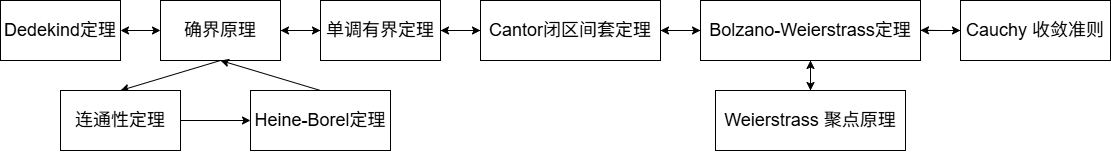
\includegraphics[width=1.0\linewidth]{figure/C2/111}
\end{center}
下面我们列举出其他的一些证明
\begin{proposition}
	用Cantor闭区间套定理证明确界原理
\end{proposition}
\begin{proof}
	
	设 $S$ 是非空有上界的实数集合，又设 $T$ 是由 $S$ 的所有上界所组成的集合，现证 $T$含有最小数，即 $S$ 有上确界．
	
	取 $a_1 \notin T, b_1 \in T$ ，显然 $a_1<b_1$ ．现按下述的规则依次构造一列闭区间：
	
	$$
	\begin{aligned}
		& {\left[a_2, b_2\right]= \begin{cases}{\left[a_1, \dfrac{a_1+b_1}{2}\right],} & \text { 若 } \dfrac{a_1+b_1}{2} \in T, \\
				{\left[\dfrac{a_1+b_1}{2}, b_1\right],} & \text { 若 } \dfrac{a_1+b_1}{2} \notin T ;\end{cases} } \\
		& {\left[a_3, b_3\right]= \begin{cases}{\left[a_2, \dfrac{a_2+b_2}{2}\right],} & \text { 若 } \dfrac{a_2+b_2}{2} \in T, \\
				{\left[\dfrac{a_2+b_2}{2}, b_2\right],} & \text { 若 } \dfrac{a_2+b_2}{2} \notin T ;\end{cases} }
	\end{aligned}
	$$
	
	$$\cdots$$
	
	由此得到一个闭区间套 $\left\{\left[a_n, b_n\right]\right\}$ ，满足
	
	$$
	a_n \notin  T, b_n \in T, \quad n=1,2,3, \cdots
	$$
	
	
	由闭区间套定理，存在惟一的实数 $\xi$ 属于所有的闭区间 $\left[a_n, b_n\right]$ ，且 $\lim\limits_{n \rightarrow \infty} a_n=\lim\limits _{n \rightarrow \infty} b_n=\xi$ ．现只需说明 $\xi$ 是集合 $T$ 的最小数，也就是集合 $S$ 的上确界．
	
	若 $\xi \notin T$ ，即 $\xi$ 不是集合 $S$ 的上界，则存在 $x \in S$ ，使得 $\xi<x$ ．由 $\lim\limits_{n \rightarrow \infty} b_n=\xi$ ，可知当 $n$ 充分大时，成立 $b_n<x$ ，这就与 $b_n \in T$ 发生矛盾，所以 $\xi \in T$ ．
	
	若存在 $\eta \in T$ ，使得 $\eta<\xi$ ，则由 $\lim\limits_{n \rightarrow \infty} a_n=\xi$ ，可知当 $n$ 充分大时，成立 $\eta<a_n$ ．由于 $a_n \in T$ ，于是存在 $y \in S$ ，使得 $\eta<a_n<y$ ，这就与 $\eta \in T$ 发生矛盾．从而得出 $\xi$ 是集合 $S$ 的上确界的结论．确界存在定理得证．
	
\end{proof}

\begin{proposition}
	确界原理证明有限覆盖定理
\end{proposition}

\begin{proof}
	构造集合 $S = \{x | a < x \leqslant b, [a, x]$ 能被 $H$ 中有限个开区间覆盖 $\}$；显然 $S$ 有上界,因 $H$ 覆盖闭区间 $[a, b]$,所以存在一个开区间 $(\alpha, \beta) \in H$ 使 $a \in (\alpha, \beta)$ .取 $x \in (\alpha, \beta)$ ,则 $[a, x]$ 能被 $H$ 中有限个开区间覆盖,从而 $x \in S$ ,故 $S$ 非空；

由确界原理存在 $\xi = \sup S$ ,现证 $\xi = b$ .用反证法.若 $\xi \neq b$ ,则 $a < \xi < b$ ,由 $H$ 覆盖闭区间 $[a, b]$,一定存在 $(\alpha_1, \beta_1) \in H$,使 $\xi \in (\alpha_1, \beta_1)$ .取 $x_1, x_2$ 使 $\alpha_1 < x_1 < \xi < x_2 < \beta_1$ ,且 $x_1 \in S$ ,则 $[a, x_1]$ 能被 $H$ 中有限个开区间覆盖,把 $(\alpha_1, \beta_1)$ 加进去,就推得 $x_2 \in S$ 这与 $\xi = \sup S$ 矛盾,故 $\xi = b$ ,即定理结论成立.
\end{proof}

\begin{proposition}
	确界原理证明$Cauchy$收敛准则
\end{proposition}
\begin{proof}
	必要性是由数列收敛定义直接得到的,不需要用到其它完备性定理.下面证充分性.（后面用其他定理证明$Cauchy$收敛准则都只证充分性,不再赘叙）
	
	设 $\{x_n\}$ 是$Cauchy$列,则 $\{x_n\}$ 是有界的（这一条也与其它实数完备性定理无关,后面用其他定理证明$Cauchy$收敛准则时直接使用,不再赘叙,请读者参考教材补充完整）.定义集合
	
	$$A = \{x | \text{存在正整数} N, \text{使任意的} n > N, \text{有} x_n > x\}  $$
	
	显然对于任意取定的 $\varepsilon > 0$ 和某个充分大的 $m$,必有 $x_m - \varepsilon \in A$,$x_m + \varepsilon \notin A$（否则将推出 $\{x_n\}$ 无界）,所以 $A$ 非空且有上界.由确界原理,$A$ 有上确界,记 $\sup A = a$.我们证明 $\{a_n\}$ 收敛于 $a$.
	
	任给 $\varepsilon > 0$,因为 $a$ 是 $A$ 的确界,故 $a - \varepsilon$ 必不是 $A$ 的上界,即存在 $x$ 属于 $A$,有 $x > a - \varepsilon$,由 $A$ 的定义知存在 $N$,使得对于任意 $n > N$,有 $x_n > a - \varepsilon$；又由$Cauchy$列的定义,存在 $N'$,使得对于任意的 $n, m > N'$,有 $|x_n - x_m| < \dfrac{\varepsilon}{2}$.显然 $a + \dfrac{\varepsilon}{2}$ 不属于 $A$,故对于 $N'$,必存在 $m' > N'$,且 $x_m \leqslant a + \dfrac{\varepsilon}{2}$,$|x_n - x_{m'}| < \dfrac{\varepsilon}{2}$,故 $x_n < a + \varepsilon$.于是任给 $\varepsilon > 0$,当 $n > \max\{N, N'\}$ 时,总有 $|x_n - a| < \varepsilon$,这就证明了$Cauchy$序列必定是收敛的.
\end{proof}
\begin{proposition}
	单调有界定理证明致密性定理
\end{proposition}
\begin{proof}
	
设 $S$ 是一有界无限点集,则在 $S$ 中可选取可数多个互不相同的点组成数列 $\{a_n\}$,显然数列 $\{a_n\}$ 是有界的.下面我们从 $\{a_n\}$ 中抽取一个单调子列,从而由单调有界定理该子列收敛,最后我们证明该子列的极限值,就是有界无限点集 $S$ 的聚点.

分两种情况来讨论：$(1)$ 如果在 $\{a_n\}$ 的任意一项之后,总存在最大的项,设 $a_1$ 后的最大项是 $a_{n_1}$,而 $a_{n_1}$ 后的最大项是 $a_{n_2}$,则显然 $a_{n_2} \leqslant a_{n_1}$.一般地,$a_{n_k}$ 后的最大项记为 $a_{n_{k+1}} (\leqslant a_{n_k}, k = 1, 2, \cdots)$.这样,就得到了 $\{a_n\}$ 的一个单调递减的子列 $\{a_{n_k}\}$,因为 $\{a_n\}$ 有界,由单调有界定理知,$\{a_{n_k}\}$ 收敛.

$(2)$. 如果 $(1)$ 不成立, 即从某一项以后, 任何一项都不是最大的, 由于前有限项不影响结果, 不妨设从第一项起, 每一项都不是最大项. 于是, 取 $a_{n_1} = a_1$ , 因 $a_{n_1}$ 不是最大项, 所以还存在另一项 $a_{n_2} > a_{n_1} (n_2 > n_1)$ , 又因为 $a_{n_2}$ 也不是最大项, 所以又有$a_{n_3} > a_{n_2} (n_3 > n_2)$ 这样一直作下去,就得到 $\{a_n\}$ 的一个单调递增子列 $\{a_{n_k}\}$,且这个子列有上界,由单调有界定理知,$\{a_{n_k}\}$ 收敛.

总之,不论 $\{a_n\}$ 属于情形 $(1)$ 还是情形 $(2)$,都可作出 $\{a_n\}$ 的一个单调收敛的子列.
\end{proof}




\begin{proposition}
	区间套定理证明确界原理
\end{proposition}

\begin{proof}
	只证明非空有上界的数集 $S$ 必有上确界,有下界的数集类似可证.

取 $S$ 的上界为 $b$ ,且 $b \notin S$ ；取 $a \in S$ ,且 $a$ 不是 $S$ 的上界,则 $a < b$ .

设闭区间 $[a_1, b_1] = [a, b]$. 

$Step\ 1$：取 $[a_1, b_1]$ 的中点 $\dfrac{a_1 + b_1}{2}$,若其是数集 $S$ 的上界,则取 $[a_2, b_2] = \left[a_1, \dfrac{a_1 + b_1}{2}\right]$；若不是数集 $S$ 的上界,则取 $[a_2, b_2] = \left[\dfrac{a_1 + b_1}{2}, b_1\right]$.

$Step\ 2$：取 $[a_2, b_2]$ 的中点 $\dfrac{a_2 + b_2}{2}$,若其是数集 $S$ 的上界,则取 $[a_3, b_3] = \left[a_2, \dfrac{a_2 + b_2}{2}\right]$；若不是数集 $S$ 的上界,则取 $[a_3, b_3] = \left[\dfrac{a_2 + b_2}{2}, b_2\right]$.

以此类推,

$Step\ n$：取 $[a_n, b_n]$ 的中点 $\dfrac{a_n + b_n}{2}$,若其是数集 $S$ 的上界,则取 $[a_{n+1}, b_{n+1}] = \left[a_n, \dfrac{a_n + b_n}{2}\right]$；若不是数集 $S$ 的上界,则取 $[a_{n+1}, b_{n+1}] = \left[\dfrac{a_n + b_n}{2}, b_n\right]$.

无限进行下去,易知

$$\lim\limits_{n \to \infty} (b_n - a_n) = \lim_{n \to \infty} \frac{b - a}{2^n} = 0. $$

(注意上述极限是$Archimedes$性质的一个等价命题) 则满足区间套定理,于是存在 $\xi \in \mathbb{R}$,有 $\xi \in \bigcap_{i=1}^{\infty} [a_i, b_i]$,且

$$\lim_{n \to \infty} b_n = \lim_{n \to \infty} a_n = \xi. $$

任取 $x \in S$ ,由二分法知 $x \leqslant b_n$ ,从而 $x \leqslant \lim\limits_{n \to \infty} b = \xi$ ,即 $\xi$ 是数集 $S$ 的一个上界.又由 $\lim\limits_{n \to \infty} a_n = \xi$ 知,$\forall \varepsilon > 0$,存在 $N$ ,当 $n > N$ 时,有 $a_n > \xi - \varepsilon$ .由分法知 $a_n$ 或者刚好是 $S$ 的上确界,或者不是 $S$ 的上界,则当 $n > N$ 时,存在 $x_0 \in S$ ,使得 $\xi - \varepsilon < a_n \leqslant x_0$.即 $\xi = \sup S$.
\end{proof}
\begin{proposition}
	区间套定理证明有限覆盖定理
\end{proposition}

\begin{proof}
	用反证法.假设定理的结论不成立,即不能用 $H$ 中有限个开区间来覆盖 $[a, b]$.

将 $[a, b]$ 等分为两个子区间,则其中至少有一个子区间不能用 $H$ 中有限个开区间来覆盖.记这个子区间为 $[a_1, b_1]$,则 $[a_1, b_1]\subset[a, b]$,且 $b_1-a_1=\dfrac{1}{2}(b-a)$.

再将 $[a_1, b_1]$ 等分为两个子区间,同样,其中至少有一个子区间不能用 $H$ 中有限个开区间来覆盖.记这个子区间为 $[a_2, b_2]$,则 $[a_2, b_2]\subset[a_1, b_1]$,且 $b_2-a_2=\dfrac{1}{2^2}(b-a)$.

重复上述步骤并不断地进行下去,则得到一个闭区间列 $\{[a_n, b_n]\}$,它满足

$$[a_n, b_n]\supset[a_{n+1}, b_{n+1}], n=1,2,\cdots, $$ $$b_n-a_n=\dfrac{b-a}{2^n}\to0(n\to\infty), $$

即 $\{[a_n, b_n]\}$ 是区间套,且其中每一个闭区间都不能用 $H$ 中有限个开区间来覆盖.

由区间套定理,存在唯一的一点 $\xi\in[a_n, b_n]$,$n=1,2,\cdots$.由于 $H$ 是 $[a, b]$ 的一个开覆盖,故存在开区间 $(\alpha, \beta)\in H$,使 $\xi\in(\alpha, \beta)$.于是,当 $n$ 充分大时有

$$[a_n, b_n]\subset(\alpha, \beta). $$

这表明 $[a_n, b_n]$ 只需用 $H$ 中的一个开区间 $(\alpha, \beta)$ 就能覆盖,与挑选 $[a_n, b_n]$ 时的假设“不能用 $H$ 中有限个开区间来覆盖”相矛盾.从而证得必存在属于 $H$ 的有限个开区间能覆盖$[a, b]$.

\end{proof}


\begin{proposition}
有限覆盖定理证明区间套定理
\end{proposition}

\begin{proof}
	反证法. 假设 $[a_n, b_n](n = 1, 2, \cdots)$ 没有公共点, 则 $[a_1, b_1]$ 上的任何一点都不是 $\{[a_n, b_n]\}$ 的公共点, 从而总存在一个开区间 $(x - \delta_x, x + \delta_x)$, 使得 $(x - \delta_x, x + \delta_x)$ 并非与所有的 $[a_n, b_n]$ 相交, 即存在 $[a_{n_x}, b_{n_x}]$, 使得 $[a_{n_x}, b_{n_x}]$ ∩ $(x - \delta_x, x + \delta_x) = \phi$.

现让 $x$ 取遍 $[a_1, b_1]$ 上的所有点就得到一个开区间集:

$$H = \{(x - \delta_x, x + \delta_x) | x \in [a_1, b_1]\}  $$

由有限覆盖定理, 可选出有限个开区间:

$$H' = \{(x_{k} - \delta_{x_k}, x_{k} + \delta_{x_k}) | k = 1, 2, \cdots, m\}  $$

覆盖闭区间 $[a, b]$, 其中

$$(x_{k} - \delta_{x_k}, x_{k} + \delta_{x_k}) \cap [a_{n_{x_k}}, b_{n_{x_k}}] = \phi  $$

因为 $[a_{n_{x_k}}, b_{n_{x_k}}]$ 只有有限个, 由区间套定理的条件, 它们是一个包含着一个, 因此其中一定有一个最小区间, 设为 $[a_{n_0}, b_{n_0}]$, 这时,

$$[a_{n_0}, b_{n_0}] \cap (x_{k} - \delta_{x_k}, x_{k} + \delta_{x_k}) = \phi, k = 1, 2, \cdots, m $$

从而,

$$[a_{n_0}, b_{n_0}] \cap \bigcup_{k=1}^{n} (x_{k} - \delta_{x_k}, x_{k} + \delta_{x_k}) = \phi $$

这就与 $[a_{n_0}, b_{n_0}] \subset [a_1, b_1]$ 矛盾. 所以 $[a_n, b_n](n = 1, 2, \cdots)$ 应有公共点.

\end{proof}
\begin{proposition}
	有限覆盖定理证明$Cauchy$收敛准则
\end{proposition}

\begin{proof}
	反证法.假设$Cauchy$列 ${x_n}$ 不收敛.已知 ${x_n}$ 为有界数列,而且 ${x_n}$ 是无穷点集（若 ${x_n}$ 是有限集,显然是收敛的）.

即存在闭区间 $[a, b]$ 使得 $\{x_n\} \subset [a, b]$. 则 $\forall x \in [a, b]$, $\exists U(x), \delta$ 使得 $U(x, \delta)$ 中只含有 $\{x_n\}$ 中的有限多项 (否则, 若 $\forall \delta > 0, U(x, \delta)$ 都有 $\{x_n\}$ 中的无限多项, 则易证 $\{x_n\}$ 收敛, 这与假设矛盾).

从而得 $[a, b]$ 的一个开覆盖 $H = \{U(x, \delta) | x \in [a, b]\}$, 由有限覆盖定理, 存在 $H$ 的一个有限子覆盖

$$H' = \{U(x_i, \delta_i) | x_i \in [a, b], i = 1, 2, \cdots, k\}, $$

所以 $\bigcup_{i=1}^{k} U(x_i, \delta_i)$ 只含有 $\{x_n\}$ 中的有限多个点, 这显然与 $\bigcup_{i=1}^{k} U(x_i, \delta_i) \supset [a, b] \supset \{x_n\}$ 矛盾. 因此 $\{x_n\}$ 必收敛.

\end{proof}


\begin{proposition}
	聚点定理证明确界原理
\end{proposition}

\begin{proof}
	设 $S$ 是非空有上界的数集.有限集时显然有上确界,不妨假设 $S$ 是无穷集合.

又设 $M$ 是 $S$ 的一个上界,如果 $M \in S$ 或者 $M$ 是 $S$ 的聚点（如果 $S$ 有聚点的话）,则 $M = \sup S$ ,定理成立.因此,下面假设 $M \in S$ 且 $M$ 不是 $S$ 的聚点.

在 $S$ 中任取一 $x_0$ ,总有 $x_0 < M$ ,考虑区间 $[x_0, M]$：

或者 $[x_0, M]$ 上只有 $S$ 的有限多个点,这时定理显然成立；或者 $[x_0, M]$ 上有 $S$ 的无穷多个点,那么, $S$ 在 $[x_0, M]$ 上的无穷多个点组成一有界的无穷点集.根据聚点原理, $S$ 在 $[x_0, M]$ 上必有聚点.

$(1)$ 若 $S$ 在 $[x_0, M]$ 上的聚点唯一,定理一定成立

事实上,若这个唯一聚点是 $x_0$ ,任取一个 $x_1 \in [x_0, M] \cap S$ ,则在 $[x_0, M]$ 上只能有 $S$ 的有限多个点（否则, $S$ 在 $[x_0, M]$ 上还有聚点,这与 $S$ 在 $[x_0, M]$ 上的聚点唯一相矛盾）,这时定理成立；

若这个唯一聚点是 $[x_0, M]$ 的内点 $\xi$ ,要么 $\xi$ 点的右边没有 $S$ 中的点,这时 $\xi = \sup S$ ,要么 $\xi$ 点右边还有 $S$ 中的点 $x_2$ ,那么在 $[x_2, M]$ 上只能有 $S$ 的有限多个点,其中最大者就是 $\sup S$ ,定理成立.

$(2)$ 若 $S$ 在 $(x_0, M)$ 上的聚点不是唯一的.

先证明下列结论成立：在 $(x_0, M)$ 内总存在一点 $x$ ,使得 $S$ 在 $[x, M]$ 上的聚点有且仅有一个.

假定这个结论不成立,那就是说对 $(x_0, M)$ 内的任意一点 $x$,或者在 $[x, M]$ 上总没有 $S$ 的聚点,或者在 $[x, M]$ 上总有 $S$ 的多个聚点.

如果前种情况发生,则根据 $x \in (x_0, M)$ 的任意性知 $(x_0, M)$ 内的任何内点都不是 $S$ 的聚点（因为假定有 $\xi \in [x_0, M]$ 是 $S$ 的聚点,则总有 $x_0 < x' < \xi < M$,于是 $[x', M]$ 上就有 $S$ 的聚点,这与在 $[x_0, M]$ 内的任意一点 $x$,$[x, M]$ 上总没有 $S$ 的聚点相矛盾）.与 $S$ 在 $(x_0, M)$ 上的聚点不是唯一的前提相矛盾.

如果后种情况发生,根据r的任意性推知$M$必是$S$的聚点,这又与前面“$M$不是$S$的聚点”的假设相矛盾.所以,上述结论必成立.

既然在 $(x_0, M)$ 内总存在一点 $x$,使得 $S$ 在 $[x, M]$ 上的聚点唯一,那么根据前面的讨论,定理成立.
\end{proof}

\begin{proposition}
	致密性定理证明有限覆盖定理
\end{proposition}

\begin{proof}
	设 $H$ 为 $[a, b]$ 的一个开覆盖,假设 $H$ 不存在有限子覆盖,则对 $[a, b]$ 二等分作区间套 $\{[a_n, b_n]\}$,使得每个 $[a_n, b_n]$ 都不存在有限子覆盖.

根据闭区间套的做法知,$\{b_n\}$ 为有界数列,故由致密性定理知,存在 $\{b_n\}$ 的子数列 $\{b_{n_k}\}$ 收敛,设 $\lim_{k \to \infty} b_{n_k} = \xi$,由 $\lim\limits_{k \to \infty} (b_{n_k} - a_{n_k}) = 0$ 知 $\lim\limits_{k \to \infty} a_{n_k} = \xi$,显然 $\xi \in [a, b]$.

由 $[a, b]$ 被 $H$ 覆盖知,存在开区间 $(\alpha, \beta) \in H$,使 $\xi \in (\alpha, \beta)$,由 $\lim_{k \to \infty} a_{n_k} = \lim\limits_{k \to \infty} b_{n_k} = \xi$ 知,存在充分大的 $K$ 使得 $[a_{n_K}, b_{n_K}] \subset (\alpha, \beta)$,这与 $[a_{n_K}, b_{n_K}]$ 不能被 $H$ 有限覆盖矛盾.故 $H$ 必有有限子覆盖.
\end{proof}


\begin{proposition}
	 $Cauchy$ 收敛准则证明单调有界定理
\end{proposition}

\begin{proof}
	设 $\{x_n\}$ 为递增有上界数列,下面我们用反证法证明数列 $\{x_n\}$ 有极限.假设 $\{x_n\}$ 不存在极限.由$Cauchy$ 收敛准则,$\exists \varepsilon_0 > 0, \forall N, \exists n > N$, 使得 $x_n - x_N = |x_n - x_N| > \varepsilon_0$.

依次取 $N_1 = 1, \exists n_1 > N_1$ 使得 $x_{n_1} - x_1 > \varepsilon_0$;

$$N_2 = n_1, \exists n_2 > n_1 \text{使得} x_{n_2} - x_{n_1} > \varepsilon_0; $$ $$\vdots $$ $$N_k = n_{k-1}, \exists n_k > n_{k-1} \text{使得} x_{n_k} - x_{n_{k-1}} > \varepsilon_0. $$

把以上式子相加得 $x_{n_k} - x_1 > k \varepsilon_0$,对任意的实数 $G$,当 $k > \dfrac{G - x_1}{\varepsilon_0}$ 时有 $x_{n_k} > G$,这与 $\{x_n\}$ 有上界矛盾.故数列 $\{x_n\}$ 有极限.

\end{proof}
\begin{proposition}
	$Cauchy$ 收敛准则证明致密性定理

\end{proposition}
\begin{proof}
	设 $S$ 是直线上的有界无限点集,所以 $\exists M > 0$,对任意的 $x \in S$ 都有 $-M \leqslant x \leqslant M$.

令 $[a_1, b_1] = [-M, M]$,则 $[a_1, b_1]$ 中含有 $S$ 的无穷多个点.

将 $[a_1, b_1]$ 二等分为两个小区间,则其中至少有一个闭区间含有 $S$ 的无穷多个点,记这样的小闭区间为 $[a_2, b_2]$.这样无限进行下去,得一闭区间套 $\{[a_n, b_n]\}$,每一个闭区间 $[a_n, b_n]$ 中都含有 $S$ 的无穷多个点.因此,存在 $x_1 \in S$ 使 $x_1 \in [a_1, b_1]$ ,存在 $x_2 \in S$ 使 $x_2 \in [a_2, b_2]$ 且 $x_2 \neq x_1$ ,一般地,存在 $x_n \in S$ 使 $x_n \in [a_n, b_n]$ 且 $x_n \notin {x_1, x_2, \cdots, x_{n-1}}$.

下面证明数列 $\{x_n\}$ 满足$Cauchy$收敛准则.

$\forall 0 < \varepsilon < 1$,取$N = \dfrac{\dfrac{\ln M}{\varepsilon}}{\ln 2}$,当 $m, n > N$ 时,有$x_m, x_n \in [a_{N+1}, b_{N+1}]$,则

$$|x_m - x_n| \leqslant b_{N+1} - a_{N+1} = \dfrac{M}{2^N} = \varepsilon  $$

故由$Cauchy$收敛准则知,数列 $\{x_n\}$ 收敛,设 $\lim\limits_{n \to \infty} x_n = \xi$.

\end{proof}










%
